\section{Characterization Problem Results}
\label{sec:CharResults}

To quantify the $\Omega$-method success for a variety of anisotropy-inducing
physics, we will present various forms of the Figure of Merit, as described in
Section \ref{sec:successmetrics}.
In the preceding subsections, a
subset of flux anisotropy-inducing physics have been identified
and a subset of problems that contain these physics have been conceived.
In this section, the results for CADIS-$\Omega$, CADIS, and nonbiased Monte Carlo
will be presented for each of these problems. Explanations on the performance of
the $\Omega$ methods will accompany the results for each problem. In some cases,
variants of problems were run to confirm or refute observations seen
in other problems.

\subsection{Computational Specifications}
\label{subsec:comp_specs}

As noted in a number of the previous sections, hybrid methods require both a
deterministic and a Monte Carlo calculation to obtain a problem result. These
transport codes require different computational parameters to obtain an answer.
For the characterization problems the computational parameters are summarized in
Table \ref{tab:simulation_defaults}; the parameters for the deterministic and
Monte Carlo calculations are demarcated in the table.

\begin{table}[h!]
  \centering
  \begin{tabular}{l|m{5cm}}
\toprule
Parameter Type & Parameter Value \\
\midrule \midrule
\multicolumn{2}{c}{ADVANTG Values$^1$} \\
\midrule
P$_N$ Order               &    $3$ \\
Quadrature Type           &  Quadruple Range \\
Quadrature Order          &    $10$ \\
Spatial Solver            &  Step Characteristic \\
Energy Group Library$^{\dagger}$     &    27G19N \\
Boundary Conditions & vacuum \\
\midrule \midrule
\multicolumn{2}{c}{MCNP Values$^2$} \\
\midrule
Particle Count      &   $1e7$ \\
Boundary Conditions & vacuum \\
\bottomrule
\end{tabular}
\begin{flushleft}
\footnotesize{
  $^1$ ADVANTG runs of the characterization problems
  were run on 16 cores of a 32 core node, with 256Gb of memory on
  an Oak Ridge National Laboratory compute cluster maintained by the Radiation
  Transport and Nuclear Systems Division. \\
  $^2$ MCNP runs of the characterization problems were run on the same
 machine, with 256Gb of memory but using all 32 cores of the node. \\
  $^{\dagger}$ Parameter type that has no default in ADVANTG.}
\end{flushleft}


  \caption[Default simulation values for characterization problems.]{
    Default simulation values for the characterization problems. The values for
    ADVANTG primarily signify parameters used to run Denovo, with exceptions for
    calculating biasing parameters, which is done exclusively in ADVANTG.
    MCNP-specific values are those used for Monte Carlo runs.
  }
  \label{tab:simulation_defaults}
\end{table}

The first portion of the table summarizes the values used by ADVANTG. Note that
these values all pertain to the Denovo deterministic solver, which is set up by
ADVANTG. The parameter types marked with a dagger have no default in ADVANTG.
We have chosen to use a relatively course 27 group energy group library.
Because the characterization problems are meant to identify the method's
performance pertaining to flux anisotropy, and we expect the energy group
structure to have less of an effect on anisotropy conditions than other
parameters, we opted for a
computationally inexpensive energy group mesh for the deterministic solver.
Further, this group library was designed for radiation shielding applications,
so it applies to the majority of the characterization problems.

The boundary conditions for all of the characterization problems will be vacuum.
At this time, ADVANTG does not support reflective or mirror boundary conditions
so this is a limitation in application space that we cannot address at this
time. The Monte Carlo code we use does support vacuum boundary conditions, but a
discrepancy in boundary conditions between deterministic and Monte Carlo
calculations would result in the simulation of a fundamentally different problem.

Unless noted, the values in this subsection of the table are ADVANTG
default values. They are a good initial choice for characterization of the
method because they are often chosen as the parameters for hybrid methods studies
by experienced and inexperienced ADAVANTG users.
Further, these values are defaults in ADVANTG for their
computational stability, such as not having negative valued weights or fluxes,
stable convergence, a relatively fast time to a solution, et cetera. Due to
the good properties exhibited by the solver options and because users first
using the $\Omega$-methods are likely to choose these values, the values in
Table \ref{tab:simulation_defaults} will be used for the characterization of the
$\Omega$-methods.

The latter section of the table summarizes the Monte Carlo code MCNP values for
each of the problems. The value of $1e7$ particles as a particle cutoff
was chosen because it made the
error bins in the majority of the nonbiased Monte Carlo
characterization problems less than 100\%. In some problems that are
extraordinarily difficult for Monte Carlo to solve without biasing, there were
tally bins with very high errors. In the following subsections they will be
clearly indicated and their results will not be plotted so as to not obfuscate
the CADIS and CADIS-$\Omega$ results. Time cutoffs were not chosen because
we decided to measure how effective the $\Omega$ methods were at reducing the
variance per particle. Depending on the flux maps generated from CADIS and
CADIS-$\Omega$, the time to transport a finite amount of particles may vary. As
a result, the reported times from a simulation can tell us whether the method
requires more sampling than other methods in addition to how fast it takes to
reach a desired relative error.

The responses in the NaI detectors of each of
the problems was measured with an MCNP track length tally (f4). The tally was
energetically binned to match the dataset of the multigroup dataset provided in
ADVANTG, and the entire volume of the detectors were used with no spatial
binning. It should be noted that while the tally is energetically binned, Monte
Carlo transport is not discretized in space or energy like deterministic
transport. In a nonbiased analog Monte Carlo calculation, transport is
completely continuous in space, energy, and angle. In a hybrid calculation using
VR parameters from a deterministic solution, the VR parameters will be
discretized to reflect the solution obtained from the determinstic solver. As a
result, the particle's transit throughout the
problem will be a combination of sampling both continuous and discretized-energy
dependent factors. Consider a particle that goes through a scattering event
in shielding material. In this scattering event, the particle samples from a
continuous-energy cross section and changes direction based on its energy.
However, depending on how much energy it loses in the scattering event it may
cross into the energy range of a lower-energy weight window and will require
further sampling.

All characterization problems were run on Remus, a machine operated and
maintained by the Radiation Transport and Nuclear Systems Division at Oak Ridge
National Laboratory. The ADVANTG runs were run on 16 cores of a 32 core node,
with 256Gb of memory. The MCNP runs were run on the same machine, with 256Gb of
memory but using all 32 cores of the node.

Each problem presented in Section \ref{sec:CharResults} will
use the values specified in Table \ref{tab:simulation_defaults}
unless otherwise noted.
Times to transport the Monte Carlo particle quantity varies between methods
due to differences in sampling. Monte Carlo and ADVANTG
inputs and directions on how to acquire them are
provided in Appendix \ref{sec:github_codes}.

\subsection{Single Turn Labyrinth}
\label{subsec:maze2}

The analysis of the characterization problems begins with the single turn
labyrinth.
The single turn labyrinth FOM results are summarized in Table \ref{tab:maze2foms},
and are illustrated in Figures \ref{fig:maze2result} and \ref{fig:maze2error}.
The table has six FOM values for CADIS and CADIS-$\Omega$ results, and three FOM
values for the analog (nonbiased) Monte Carlo results. The equations to
calculate each of these FOMS is summarized in Table \ref{tab:fom_defaults}.

\begin{table}[h!]
  \centering
  \begin{tabular}{lrrrrr}
\toprule
{} & \multicolumn{2}{c}{CADIS}   & \multicolumn{2}{c}{CADIS-$\Omega$}  & analog \\
{} &    MC & MC$_{hybrid}$ &         MC & MC$_{hybrid}$ &     MC \\
\midrule
tally avg   &  18.6 &        14.9 &       2.36 &        1.56 &   17.4 \\
max RE      &  2.76 &        2.21 &      0.481 &       0.318 & 0.0857 \\
min RE      &   249 &         200 &        196 &         130 &    -- \\
time (mins) &  67.7 &        84.4 &        157 &         237 &   11.7 \\
\bottomrule
\end{tabular}

  \caption[Figure of Merit comparison for single turn maze.]{Figure of Merit
    comparison for single turn maze.
    The relative errors used are the tally average relative error, the tally maximum relative
  error, and the tally minimum relative error; the times are total walltimes for
  the Monte Carlo calculation and the sum of the hybrid method software, the
  deterministic transport time, and the Monte Carlo calculation time.}
  \label{tab:maze2foms}
\end{table}

\begin{table}[h!]
  \centering
  \begin{tabular}{llrrr}
\toprule
          &              &          cadis &     cadisangle &         analog \\
          &              & time (minutes) & time (minutes) & time (minutes) \\
\midrule
MCNP time & total &          67.71 &         157.01 &          11.67 \\
deterministic time & advantg\_time &           0.26 &           0.28 &            -- \\
          & denovo\_time &          16.41 &          78.19 &            -- \\
          & dispose\_time &           0.01 &           0.40 &            -- \\
          & omega\_time &           0.00 &           1.61 &            -- \\
          & total &          16.67 &          80.08 &            -- \\
wall time &              &          84.38 &         237.09 &          11.67 \\
\bottomrule
\end{tabular}

  \caption[Detailed timing results for single turn maze.]
  {Detailed timing results for single turn maze.}
  \label{tab:maze2times}
\end{table}

In Table \ref{tab:maze2foms} the FOM results for CADIS, CADIS-$\Omega$, and
nonbiased Monte Carlo for the single turn maze are presented. In all cases, the
CADIS FOMs are better than those obtained by CADIS-$\Omega$. The FOMS
calculated using the tally average relative error are better in the nonbiased
analog Monte Carlo than CADIS-$\Omega$ as well. However, this is a product of
two effects: the time for the analog to run the same particle count is far
shorter than either CADIS or CADIS-$\Omega$. As a result, to obtain the same
FOM, CADIS-$\Omega$ needs to have $R_1/R_2 = \sqrt{T_2/T_1}$ (this is from
taking a ratio of the FOMs) the tally average
relative error, or ~$0.27$. Because this problem is highly scattering and many
low-energy particles can make it through the concrete labyrinth, even the analog
can have good sampling at low energies, resulting in a tally average FOM that
reaches this threshold.

Table \ref{tab:maze2times} contains more detailed timing information spent in
each of the codes for each type of problem. We can see that the Monte Carlo
runtime for CADIS-$\Omega$ is more than twice that of CADIS, and almost fifteen
times that of the nonbiased analog Monte Carlo. The time to run just the
hybrid/deterministic portion of the calculation is also four times longer for
CADIS-$\Omega$ than it is for CADIS. These disparities in runtimes have a strong
negative impact on the CADIS-$\Omega$ FOMs, which was observed in the FOM
results in Table \ref{tab:maze2foms}.

\begin{figure}[h!]
  \centering
  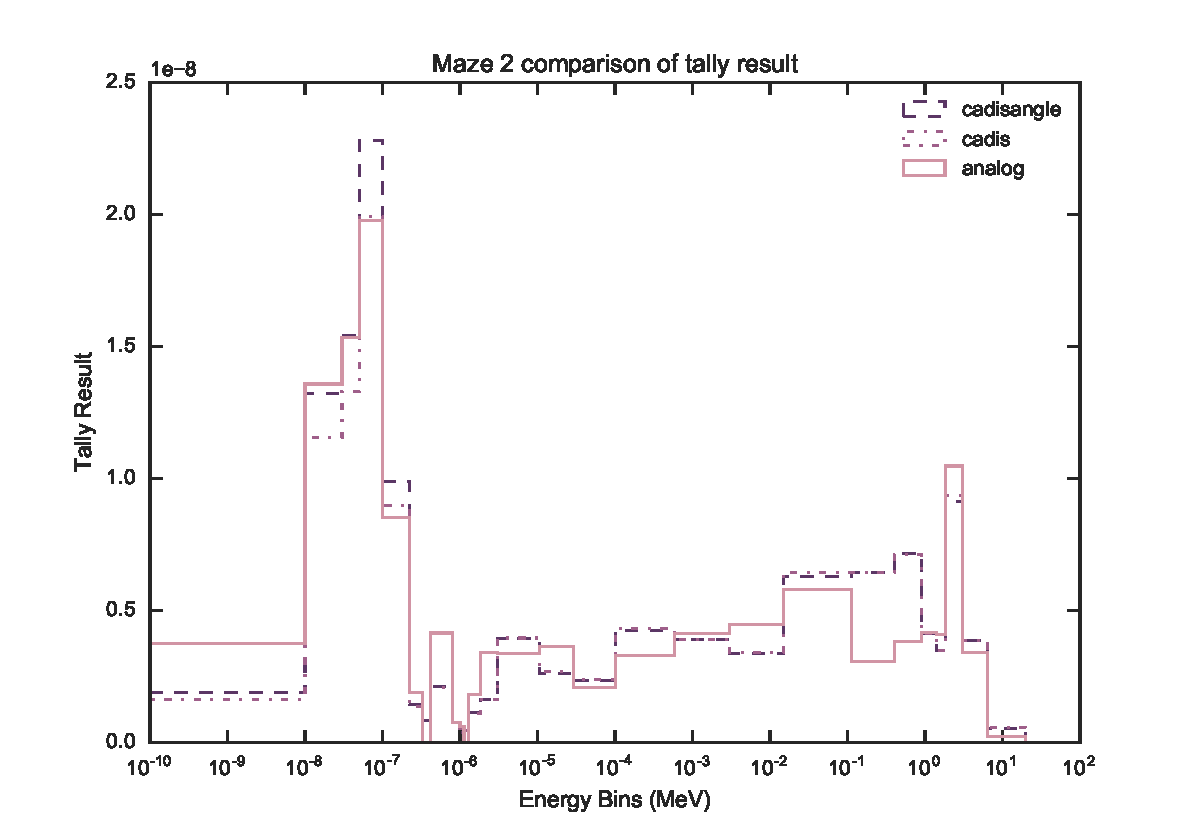
\includegraphics[height=10cm]{./chapters/characterization_probs/figures/char/maze2/maze_2_tally_result_compare.pdf}
  \caption[Tally results comparison between methods for single turn labyrinth.]
  {Tally results comparison between methods for single turn labyrinth.}
  \label{fig:maze2result}
\end{figure}

\begin{figure}[h!]
  \centering
  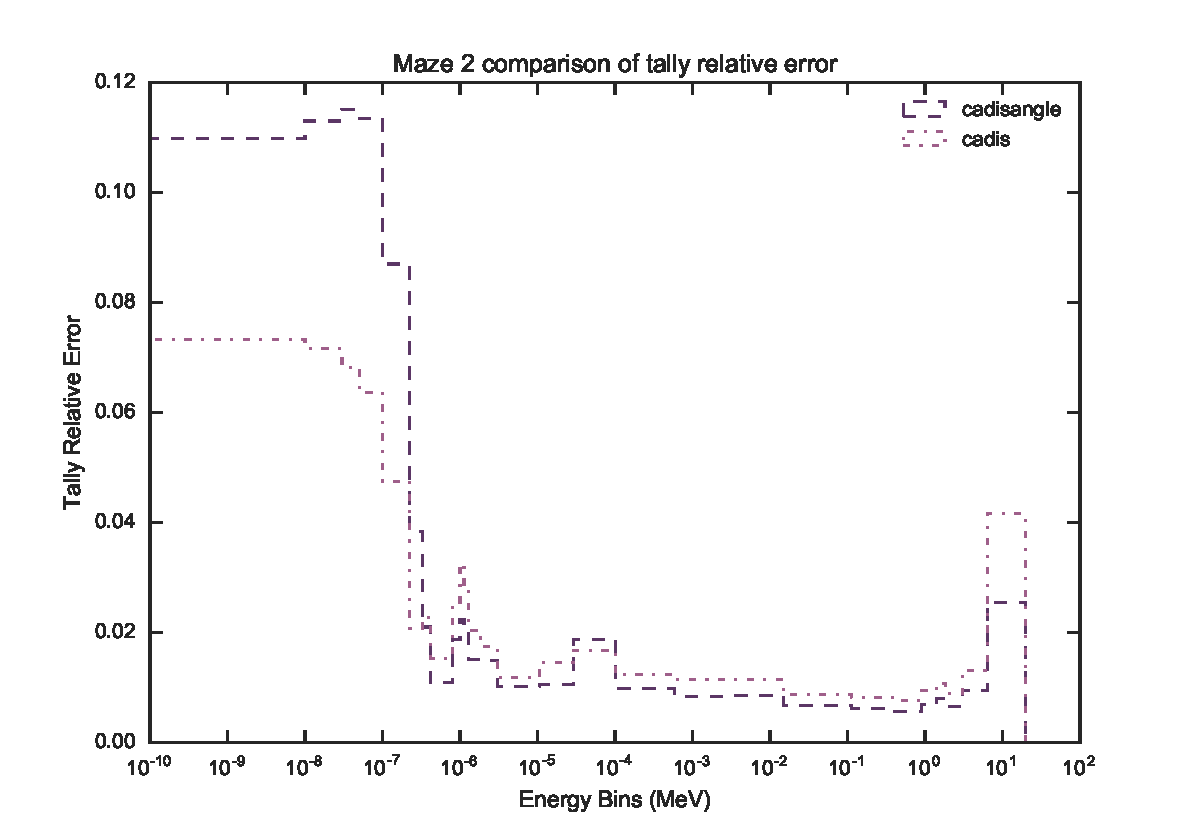
\includegraphics[height=10cm]{./chapters/characterization_probs/figures/char/maze2/maze_2_tally_error_compare.pdf}
  \caption[Tally relative error comparison between methods for single turn
  labyrinth]{Tally relative error comparison between methods for a single turn
  labyrinth.}
  \label{fig:maze2error}
\end{figure}

Figures \ref{fig:maze2result} and \ref{fig:maze2error} show the tally result and
the relative errors for each result in the single turn maze, respectively.
This particular relative error plot,
Figure \ref{fig:maze2error}, does not include the
relative error bins of the analog result because they are significantly higher
than the CADIS and CADIS-$\Omega$ results. This is further confirmed in Table
\ref{tab:maze2foms}, where the minimum relative error FOM is a non-tallied bin.

By inspecting Figure \ref{fig:maze2result}, one can observe that the CADIS and
CADIS-$\Omega$ results are in agreement in bins greater that $10^{-7}$ MeV. At
lower energy bins, CADIS-$\Omega$ generally has a higher value for the tally
result than standard CADIS. However, in comparing the errors for these low energy
bins in Figure $\ref{fig:maze2error}$, CADIS has a lower relative error. This
indicates that CADIS sampled many more low-weight particles than CADIS-$\Omega$
in these regions. Conversely, CADIS-$\Omega$ has a lower calculated relative
error than CADIS for bins greater than ~$5*10^{-6}$ MeV. This is expected, as
higher energy particles generally exhibit a stronger angular dependence than
low-energy particles. In geometric and energetic regions
where the angular dependence is stronger,
the importance map generated by CADIS-$\Omega$ may show more of an effect in
improving the relative error.

% High energy particles exiting the maze towards the tally
% detector have much longer mean free paths than the low energy particles, and
% will generally show a much stronger effect in the $\Omega$-flux in those
% regions. This is illustrated in Figure \ref{fig:}. The shape of the $\Omega$
% flux around the detector region is much more strongly dependent on direction in
% the high energy group 000 flux than it is for the lower energy group 026 flux.
% Despite having lower relative errors than CADIS at higher energies,
% CADIS-$\Omega$ has lower FOMs than CADIS for the FOMS calculated with the
% minimum relative error. As discussed previously, this is due to the long runtime
% of CADIS-$\Omega$, which is more than twice as long as CADIS. From this, we can
% conclude that while CADIS-$\Omega$ is better at transporting particles in high
% energy regions than CADIS, achieving lower relative errors, the length of time
% to do so is prohibitive and achievable by CADIS should the runtimes be the same
% for both.
%
% [todo: Omega flux lot of group 00]
%
% [todo: Omega flux plot of group 026]

\subsection{Multiple Turn Labyrinth}
\label{subsec:maze1}

The multiple turn labyrinth is built off of the single turn labyrinth geometry.
The labyrinth materials are much the same, but the geometry differs. Table
\ref{tab:maze1foms} summarizes the Figure of Merit results for CADIS,
CADIS-$\Omega$ and nonbiased Monte Carlo. Figures \ref{fig:maze1result} and
\ref{fig:maze1error} show the results obtained by the track length tally in each
method.

\begin{table}[h!]
  \centering
  \begin{tabular}{lrrrrr}
\toprule
{} & cadis &             & cadisangle &             & analog \\
{} &    MC & MC\_adjusted &         MC & MC\_adjusted &     MC \\
\midrule
tally avg   &   327 &         248 &        224 &          71 &  0.054 \\
max RE      &  1.46 &        1.11 &       1.02 &       0.322 & 0.0393 \\
min RE      &   113 &        85.6 &         71 &        22.5 &    -- \\
time (mins) &  51.5 &          68 &       35.5 &         112 &   25.5 \\
\bottomrule
\end{tabular}

  \caption[Figure of Merit comparison for multiple turn maze.]{Figure of Merit
    comparison for multiple turn maze.}
  \label{tab:maze1foms}
\end{table}

\begin{table}[h!]
  \centering
  \begin{tabular}{llrrr}
\toprule
          &              &          cadis &     cadisangle &         analog \\
          &              & time (minutes) & time (minutes) & time (minutes) \\
\midrule
MCNP time & total &          51.52 &          35.55 &          25.46 \\
deterministic time & advantg\_time &           0.25 &           0.21 &            -- \\
          & denovo\_time &          16.28 &          74.85 &            -- \\
          & dispose\_time &           0.01 &           0.40 &            -- \\
          & omega\_time &           0.00 &           1.74 &            -- \\
          & total &          16.53 &          76.80 &            -- \\
wall time &              &          68.05 &         112.35 &          25.46 \\
\bottomrule
\end{tabular}

  \caption[Detailed timing results for multiple turn maze.]
  {Detailed timing results for multiple turn maze.}
  \label{tab:maze1times}
\end{table}

In Tables \ref{tab:maze1foms} and \ref{tab:maze1times}
it is notable that the CADIS-$\Omega$ runtime is
shorter in the Monte Carlo simulation than CADIS. This differs most of the other
cases presented in this section. However, it is also notable that because the
deterministic time is so much longer for CADIS-$\Omega$, T$_{hybrid}$ ends up
being greater for CADIS-$\Omega$ than CADIS.

Table \ref{tab:maze1foms} shows that both CADIS and CADIS-$\Omega$ outperform the
analog by a factor of $10^2$ or $10^3$, indicating the necessity of variance
reduction for a problem like this. In comparing the FOMs, CADIS slightly outperforms
CADIS-$\Omega$ for all relative errors, meaning that the time
to reach any relative error will be achieved faster by CADIS.

\begin{figure}[h!]
  \centering
  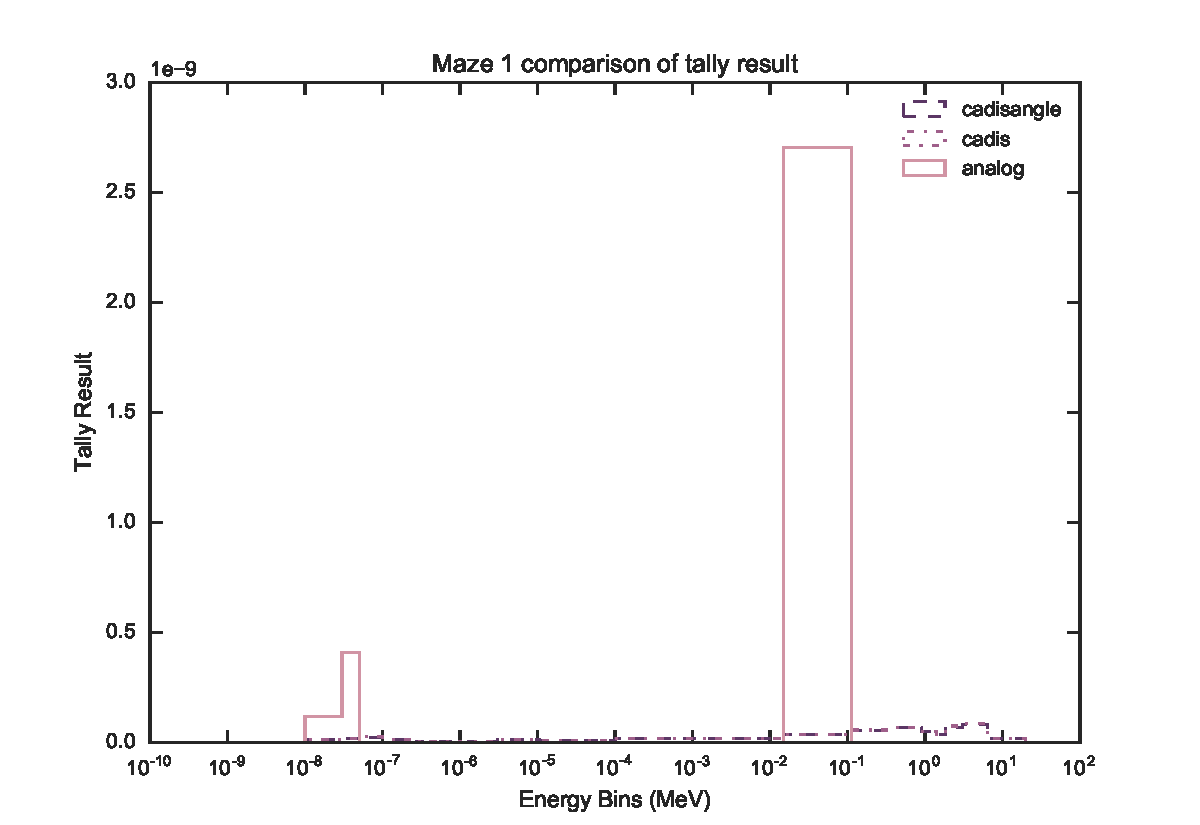
\includegraphics[height=10cm]{./chapters/characterization_probs/figures/char/maze1/maze_1_tally_result_compare.pdf}
  \caption[Tally results comparison between methods for multiple turn labyrinth.]
  {Tally results comparison between methods for multiple turn labyrinth. }
  \label{fig:maze1result}
\end{figure}

\begin{figure}[h!]
  \centering
  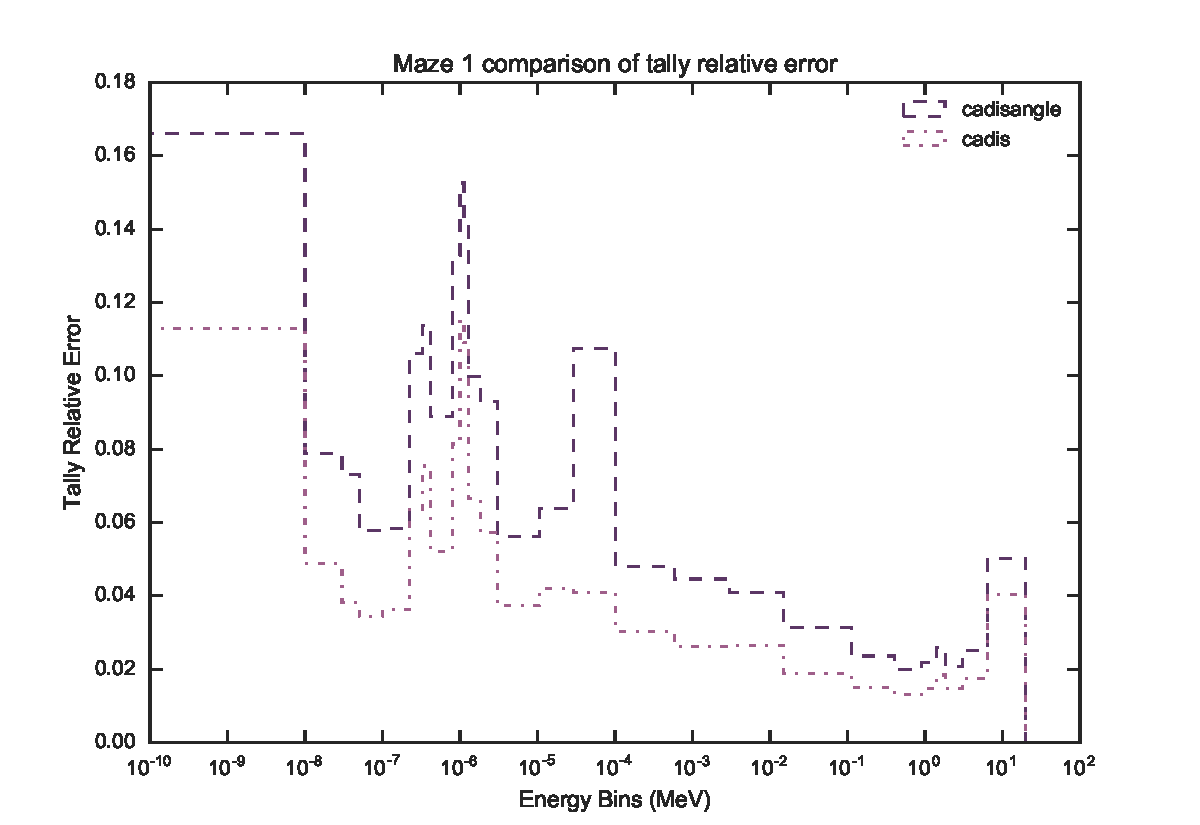
\includegraphics[height=10cm]{./chapters/characterization_probs/figures/char/maze1/maze_1_tally_error_compare.pdf}
  \caption[Tally relative error comparison between methods for multiple turn labyrinth]
  {Tally relative error comparison between methods for a multiple turn
  labyrinth. }
  \label{fig:maze1error}
\end{figure}

Looking at Figures \ref{fig:maze1result} and \ref{fig:maze1error}, we can see
that the analog Monte Carlo results differ significantly from either CADIS or
CADIS-$\Omega$. Two distinct regions of tally bins have been recorded in the
analog case: a high energy region comprised of particles that have scattered
very few times before reaching the detector, and a much smaller low energy
region, comprised of particles that are very thermal. These thermal particles
have a very small mean free path in the concrete labyrinth, thus the majority of them were
absorbed in the shield. However, given the errors on this result, these results are
not trustworthy. In the case of this problem, some of what was discussed in the
single-turn labyrinth is confirmed. This particular case requires that particles
scatter several more times if they are to exit the labyrinth from the air duct.
As a result, the spectrum is more thermal than the first case and the problem
has less anisotropy from the scattering effects.
As discussed in the single-turn labyrinth subsection, CADIS
outperformed CADIS-$\Omega$ in problems in energy bins that had less angular
dependence. Because this problem has far more scattering event, it overall has
less angular dependence and CADIS outperforms CADIS-$\Omega$ in all energy bins.
This problem is poorly suited to CADIS-$\Omega$.

In Section \ref{subsec:maze2}, it was discussed that higher energy regions that
contribute to the tally are more anisotropic, and that these regions benefit
more from the $\Omega$-flux map than they do with standard CADIS' importance
map. Using the anisotropy metrics from Section \ref{sec:anisotropy_quant}, let
us compare the anisotropy distributions of the single turn and multiple-turn
labyrinth problems. Figure \ref{fig:labyrinthviolins} are violin plots of the
M$_{3}$ distributions of the labyrinth problems. To filter out values of the
metric distribtuion that do not have a strong importance to contributing to the
tally, only values from cells above the contributon flux mean value are included
in the violins.

First, looking at the metric three distributions for both the single-
(\ref{fig:maze2M3violins})and
multiple-turn (\ref{fig:maze1M3violins}) labyrinths, we can see that the violins
in both plots shift from a fairly small grouping of values at high enrgies to a
broad range of values at low energies. The bottom of the violin in each
group also tells us a
bit about the metric distribution. Because only values from ``more important''
cells have been included in these distributions, the bottom cutoff tells us how
anisotropic the cells of median importance might be. It also tells us how many
cells have high-valued anisotropy metrics. For both the single- and
multi-turn labyrinths, we see higher-valued cutoff point in high energies than
in low energies. This indicates that more cells in high energies have higher
values of M$_3$.

\begin{figure}[htb!]
  \centering
  \begin{subfigure}[t]{\textwidth}
    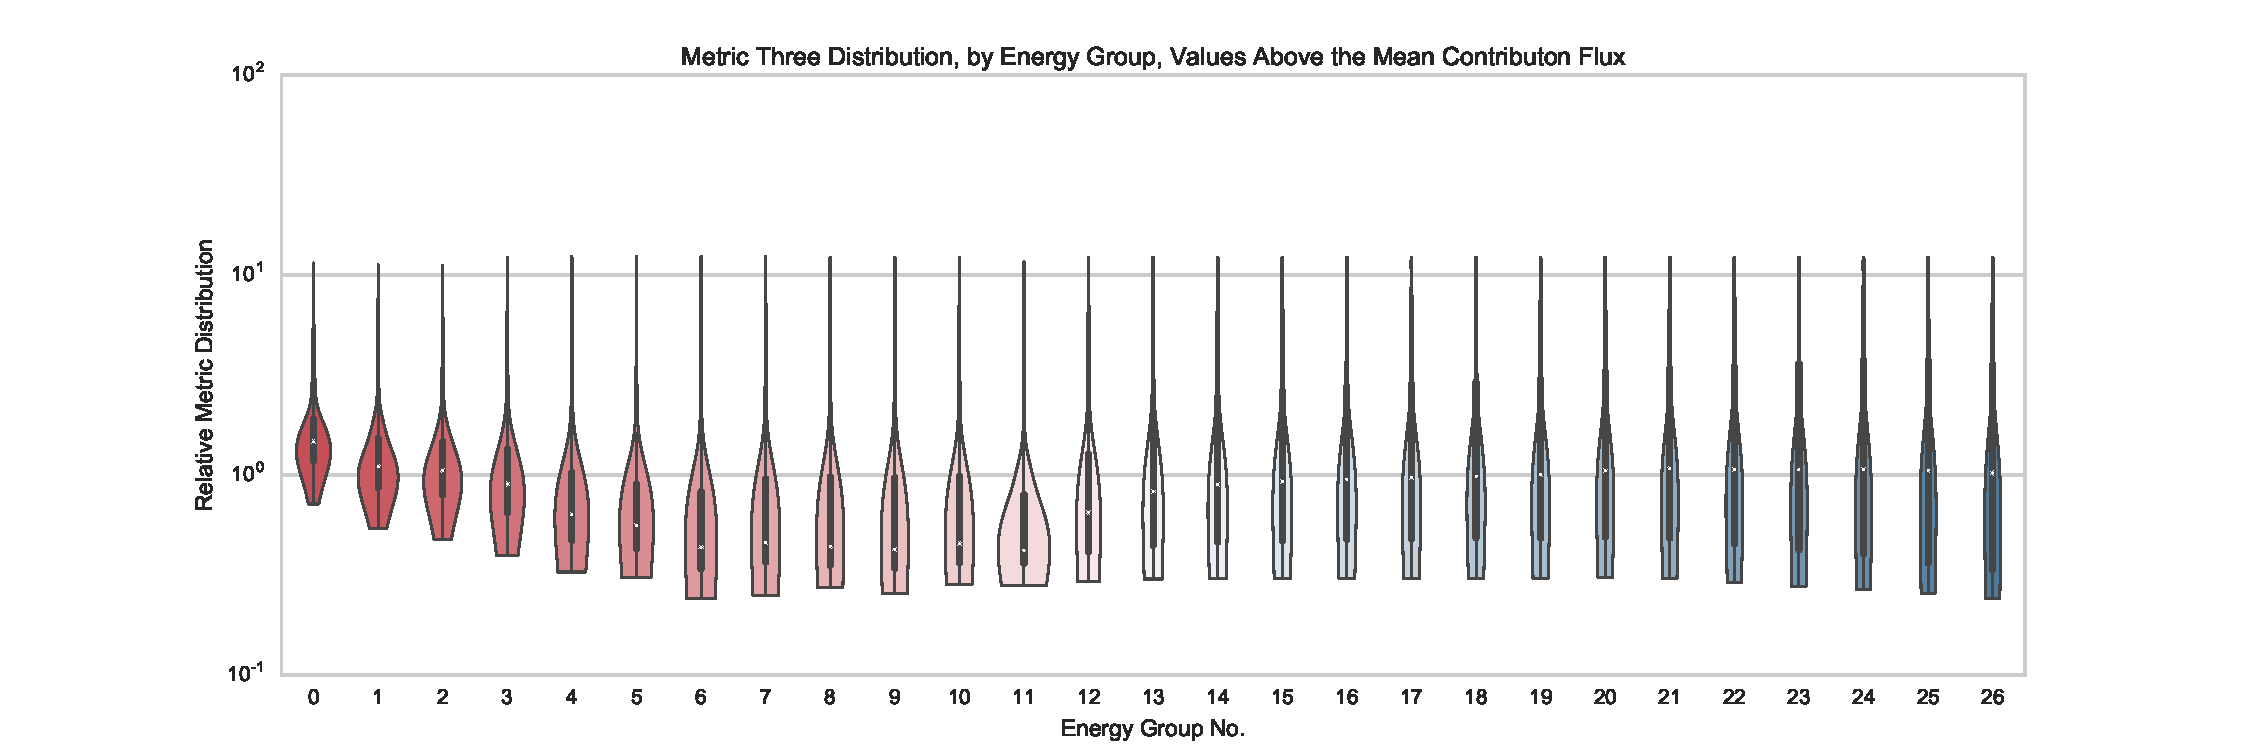
\includegraphics[width=\linewidth]{./chapters/characterization_probs/figures/char/maze2/metric_three_violin_mean.pdf}
    \caption{M$_{3}$ distribution for single turn labyrinth}
    \label{fig:maze2M3violins}
  \end{subfigure}
\end{figure}
\begin{figure}[htb!]\ContinuedFloat
  \centering
  \begin{subfigure}[t]{\textwidth}
    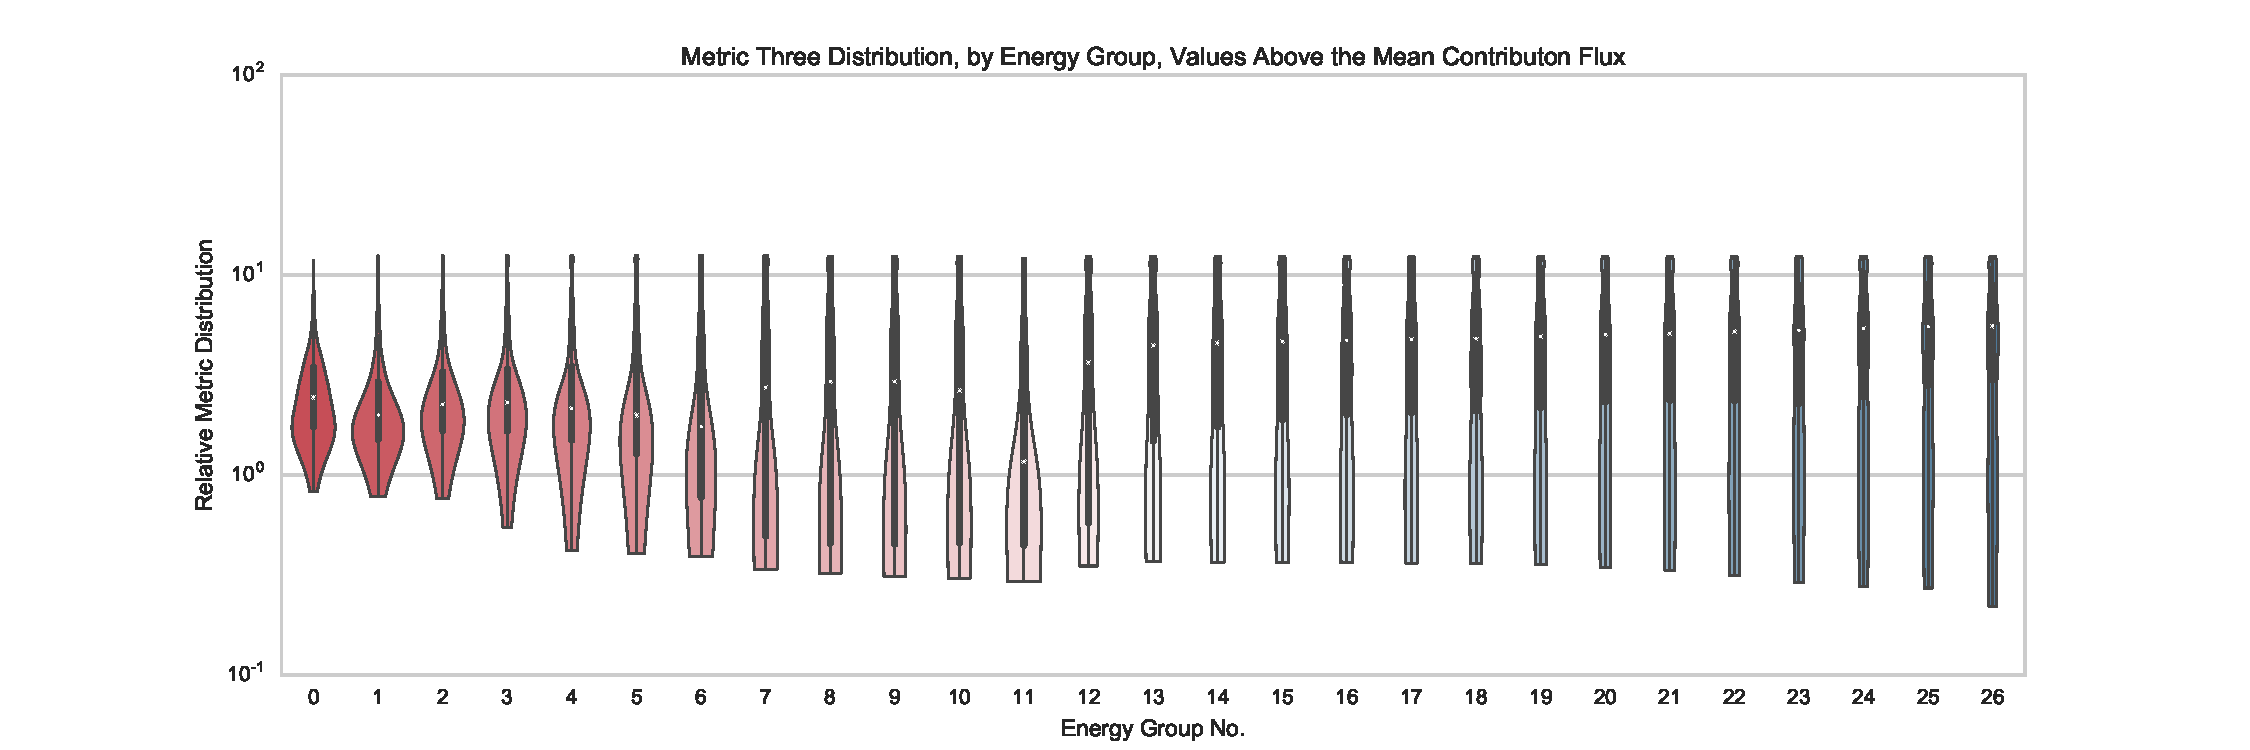
\includegraphics[width=\linewidth]{./chapters/characterization_probs/figures/char/maze1/metric_three_violin_mean.pdf}
    \caption{M$_3$ distribution for multi-turn labyrinth}
    \label{fig:maze1M3violins}
  \end{subfigure}
  \caption[Violin plots of M$_{3}$ distribution using values above the mean
  contributon flux for labyrinth problems.]
  {Violin plots of M$_{3}$ distribution using values above the mean
  contributon flux for labyrinth problems. Low energy group numbers correspond
  to high energies or fast particles, and are marked in red.}
  \label{fig:labyrinthviolins}
\end{figure}

The violin plots of the multi-turn labyrinth (Fig. \ref{fig:maze1M3violins})
tend to span a larger range of values. That is, the violins tend to be longer.
All of the violins in both plots have a bounding upper limit, meaning that in
every energy group there are some very anisotropic cells. Interestingly, it
appears that for the multi-turn labyrinth the distribution of anisotropies at
low energies has no distinctive bunching, as observed in the single-turn
labyrinth. This means that in important cells, there is an even distribution of
very anisotorpic, slightly anisotropic, and isotropic cells.

It must be noted that while
the trends in these violins are interesting, we must also be wary of using comparing
the violins directly. The filtering algorithm used to pull values out is dependent only
on the contributon flux solution for that problem, so the average contributon
flux cutoff for the single-turn labyrinth and multiple-turn labyrinth are
different. Using a raw value from the violin plot in Figure
\ref{fig:maze1M3violins} and directly comparing it to one from Figure
\ref{fig:maze2M3violins} may be misleading. Instead, this analysis will focus on
the general behavior of the metrics in each problem, not specific metric values.

\begin{figure}[htb!]
  \centering
  \begin{subfigure}[t]{\textwidth}
    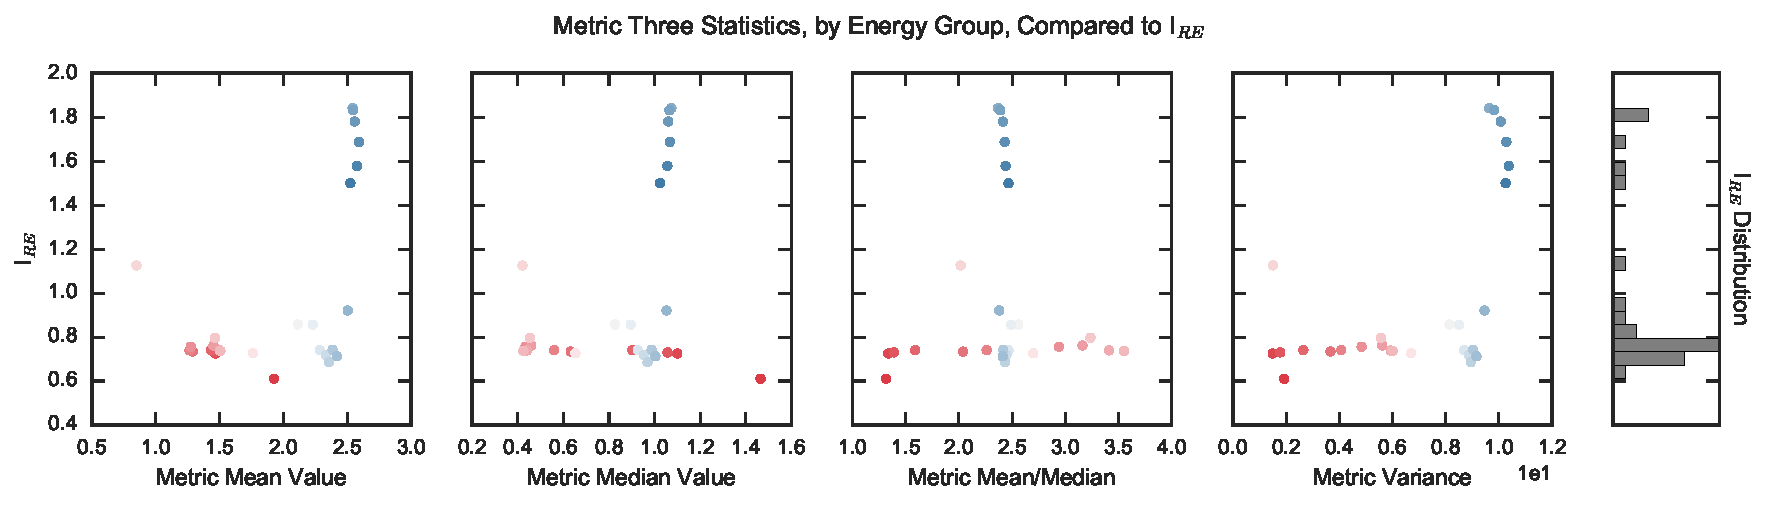
\includegraphics[width=\linewidth]{./chapters/characterization_probs/figures/char/maze2/metric_three_err_stats_mean.pdf}
    \caption{RE improvement factor as a function of M$_{3}$ statistics for single turn labyrinth}
    \label{fig:maze2M3errs}
  \end{subfigure}
\end{figure}
\begin{figure}[htb!]\ContinuedFloat
  \centering
  \begin{subfigure}[t]{\textwidth}
    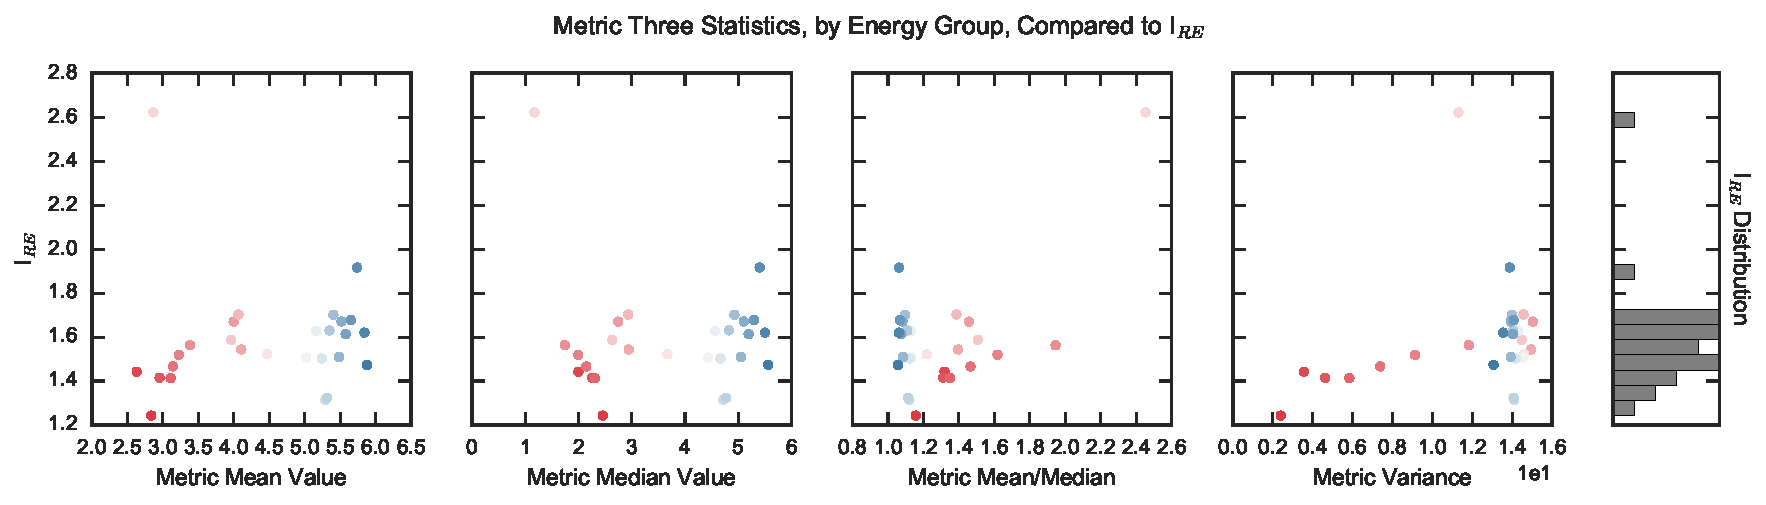
\includegraphics[width=\linewidth]{./chapters/characterization_probs/figures/char/maze1/metric_three_err_stats_mean.pdf}
    \caption{RE improvement factor as a function of M$_3$ statistics for multi-turn labyrinth}
    \label{fig:maze1M3errs}
  \end{subfigure}
  \caption[Relative error improvement factor as a function of M$_3$
  distribution statistics.]
  {Relative error improvement factor as a function of M$_3$
  distribution statistics. Metric distribution statistics are calculated using
  values of M$_3$ in cells with contributon flux values above the mean. Colors
  of datapoints correspond to the energy group to which they belong.}
  \label{fig:labyrinthIREs}
\end{figure}

Figure \ref{fig:labyrinthIREs} shows the improvement factors of the relative
errors between CADIS-$\Omega$ and CADIS for the labyrinth problems. The x-axes
of the plots in Figures \ref{fig:maze2M3errs} and \ref{fig:maze1M3errs} use the
distribution statistics from the violins in Figures \ref{fig:maze2M3violins} and
\ref{fig:maze1M3violins}, respectively. Recall that because I$_{RE}$ is the
ratio of the relative error between CADIS-$\Omega$ and CADIS--and we seek a low
relative error--that values of I$_{RE}$ below 1.0 indicate method improvement
for CADIS-$\Omega$.

Looking at the differences between Figures \ref{fig:maze2M3errs} and
\ref{fig:maze1M3errs}, some interesting effects can be observed. Recall from the
relative error distribution plots for each problem (Figures \ref{fig:maze1error} and
\ref{fig:maze2error}) that CADIS-$\Omega$ had higher relative errors in all
energy bins than CADIS for the multi-turn labyrinth, and a higher relative
error in thermal energy groups in the single-turn labyrinth.
Figure
\ref{fig:maze2M3errs} shows the isolated grouping of poorer results for low
energy bins in the single turn labyrinth. The rest of the values in this figure
all show improvement in the relative error, while the low-energy group show
better performance for CADIS. There is no distinct grouping in Figure
\ref{fig:maze1M3errs} because all of the CADIS-$\Omega$ relative errors are
higher than CADIS, so a distinct turnover in I$_{RE}$ does not occur.

There does not seem to be a tight
trend
observable for any measurement of the M$_3$ distribution and I$_{RE}$ in Figure
\ref{fig:maze2M3errs}, but the higher values of I$_{RE}$ generally occur in high
mean values of M$_3$ and higer variances of M$_3$. Figure \ref{fig:maze1M3errs}
also shows this trend in the metric mean and variance subplots, with a single
outlier in an intermediate energy group. It also appears that the spread of
I$_{RE}$ values does not change as a function of any of the metric values.

\begin{figure}[htb!]
  \centering
  \begin{subfigure}[t]{\textwidth}
    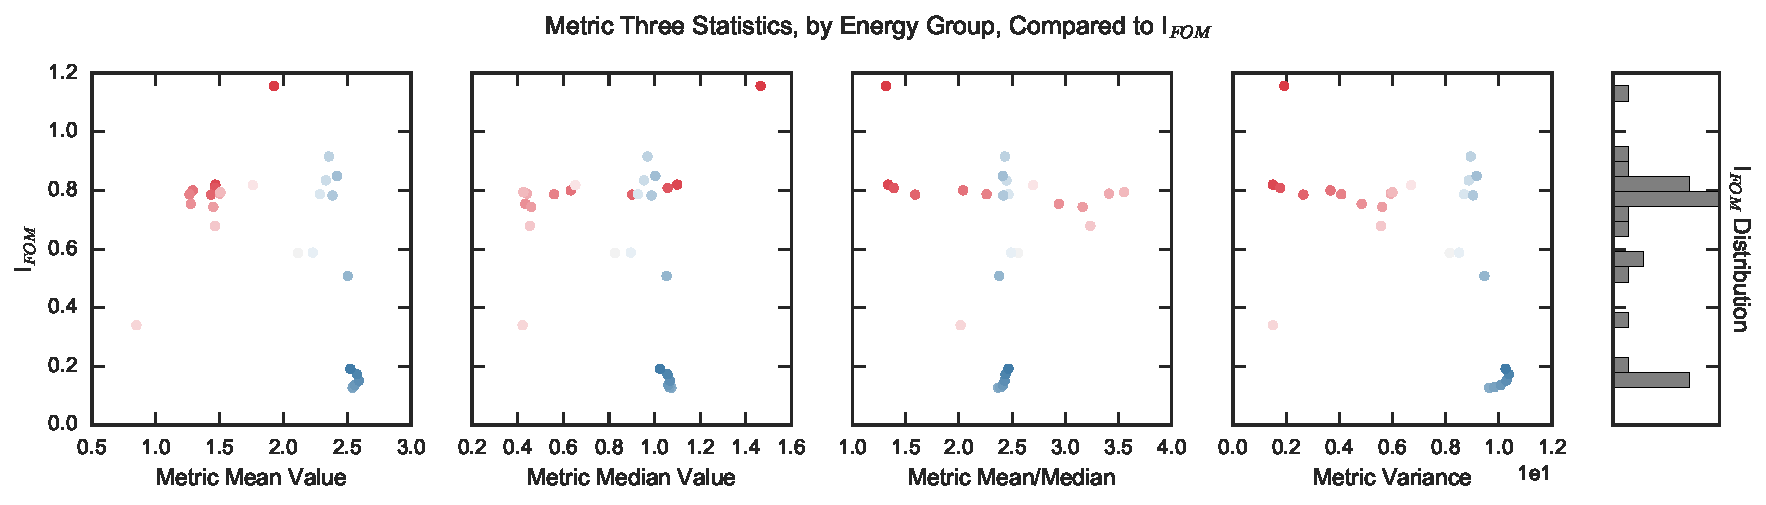
\includegraphics[width=\linewidth]{./chapters/characterization_probs/figures/char/maze2/metric_three_fom_stats_mean.pdf}
    \caption{FOM improvement factor as a function of M$_{3}$ statistics for single turn labyrinth}
    \label{fig:maze2M3FOMs}
  \end{subfigure}
\end{figure}
\begin{figure}[htb!]\ContinuedFloat
  \centering
  \begin{subfigure}[t]{\textwidth}
    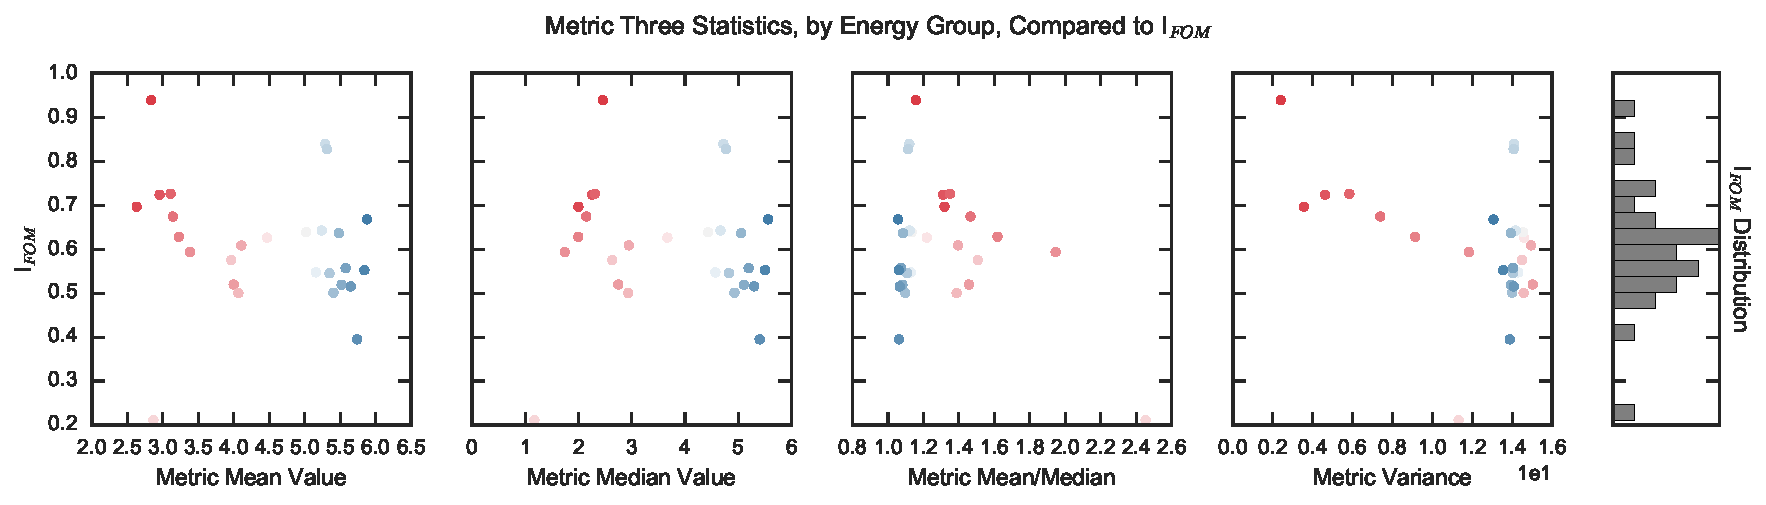
\includegraphics[width=\linewidth]{./chapters/characterization_probs/figures/char/maze1/metric_three_fom_stats_mean.pdf}
    \caption{FOM improvement factor as a function of M$_3$ statistics for multi-turn labyrinth}
    \label{fig:maze1M3FOMs}
  \end{subfigure}
  \caption[Figure of Merit improvement factor as a function of M$_3$
  distribution statistics.]
  {Figure of Merit improvement factor as a function of M$_3$
  distribution statistics. Metric distribution statistics are calculated using
  values of M$_3$ in cells with contributon flux values above the mean. Colors
  of datapoints correspond to the energy group to which they belong.}
  \label{fig:labyrinthIFOMs}
\end{figure}

Figure \ref{fig:labyrinthIFOMs} builds off of what we've already observed in Figure
\ref{fig:labyrinthIREs}. In this series of figures, I$_{FOM}$ is plotted rather
than I$_{RE}$. If CADIS-$\Omega$ has better FOM performance than CADIS, the
resulting value of I$_{FOM}$ will be above 1.0.

Many features from Figure \ref{fig:labyrinthIREs} continue in Figure
\ref{fig:labyrinthIFOMs}. The distinct grouping of low-energy results for the
single turn labyrinth are also observable in \ref{fig:maze2M3FOMs}. The intermediate
energy outlier for the multiple turn labyrinth is located at the bottom of
all of the subplots in Figure \ref{fig:maze1M3FOMs}. By adjusting our results to
include timing, even less of a trend with metric distribution measurements is
seen in the improvement metric for the single turn labyrinth. However, for the
multiple turn labyrinth it does appear that as the metric mean value increases,
I$_{FOM}$ decreases.

\subsection{Steel Beam}
\label{subsec:resultbeam}

The steel beam embedded in concrete FOM and timing
results are summarized in Tables
\ref{tab:steelbeamfoms} and \ref{tab:steelbeamtimes}. Figures
\ref{fig:steelbeamresult} and \ref{fig:steelbeamerror} show the results obtained
by the track length tally in CADIS, CADIS-$\Omega$ and the nonbiased analog
Monte Carlo.

\begin{table}[h!]
  \centering
  \begin{tabular}{lrrrrr}
\toprule
{} &    cadis &             & cadisangle &             & analog \\
{} &       MC & MC\_adjusted &         MC & MC\_adjusted &     MC \\
\midrule
tally avg   &      668 &         659 &      3e+03 &    2.96e+03 &   1.39 \\
max RE      &     3.74 &        3.69 &       6.79 &        6.71 & 0.0448 \\
min RE      & 1.43e+03 &    1.41e+03 &   1.33e+03 &    1.31e+03 &    -- \\
time (mins) &      414 &         420 &   2.09e+03 &    2.11e+03 &   22.3 \\
\bottomrule
\end{tabular}

  \caption[Figure of Merit comparison for steel bar embedded in concrete.]
  {Figure of Merit comparison for steel bar embedded in concrete. }
  \label{tab:steelbeamfoms}
\end{table}

\begin{table}[h!]
  \centering
  \begin{tabular}{llrrr}
\toprule
          &             &          CADIS & CADIS-$\Omega$ &         analog \\
        &              & \multicolumn{3}{c}{time (minutes)} \\
\midrule
MCNP time & total &         414.45 &        2086.60 &          22.33 \\
deterministic time & advantg\_time &           0.18 &           0.18 &            -- \\
          & denovo\_time &           5.69 &          25.64 &            -- \\
          & dispose\_time &           0.00 &           0.16 &            -- \\
          & omega\_time &           0.00 &           0.66 &            -- \\
          & total &           5.87 &          26.49 &            -- \\
wall time &              &         420.32 &        2113.09 &          22.33 \\
\bottomrule
\end{tabular}

  \caption[Detailed timing results for steel bar embedded in concrete.]
  {Detailed timing results for steel bar embedded in concrete.}
  \label{tab:steelbeamtimes}
\end{table}

Tables \ref{tab:steelbeamfoms} and
\ref{tab:steelbeamtimes} show that this problem is very difficult for
analog Monte Carlo and that CADIS-$\Omega$ generally performs better than CADIS.
In fact, CADIS-$\Omega$ has the best performance
in this problem of all of the characterization problems.

For both CADIS and CADIS-$\Omega$, this problem has a huge disparity in the FOMs
calculated with the maximum and minimum relative error. As a result, depending
on the convergence requirements that a user might require, the time to achieve
a desired solution could vary significantly in applications. However, both CADIS
and CADIS-$\Omega$ improve on the unbiased analog Monte Carlo's FOM by a factor
of $10^{2}$ or more.

CADIS-$\Omega$ outperforms CADIS for
the FOMS calculated with the tally average relative error and the tally maxmimum
relative error. This indicates that giving a limiting relative error to which
all energy bins must converge, CADIS-$\Omega$ will achieve it in $1/3$rd the time
that CADIS will. Further, CADIS-$\Omega$ has a better FOM than CADIS when the
deterministic runtimes are added. As shown in the timing table, the time to run
and generate the variance reduction parameters for CADIS-$\Omega$ will always be
longer than CADIS due to the addition of the forward transport run. The addition of
deterministic runtimes has the potential to lower the FOM of CADIS-$\Omega$ more than
that of CADIS, so CADIS-$\Omega$'s achievement of a FOM higher FOM with much
longer runtimes in both Monte Carlo and ADVANTG illustrates just how much lower
the relative error it achieves is. CADIS-$\Omega$ is very well-suited to a
problem with these conditions.

\begin{figure}[h!]
  \centering
  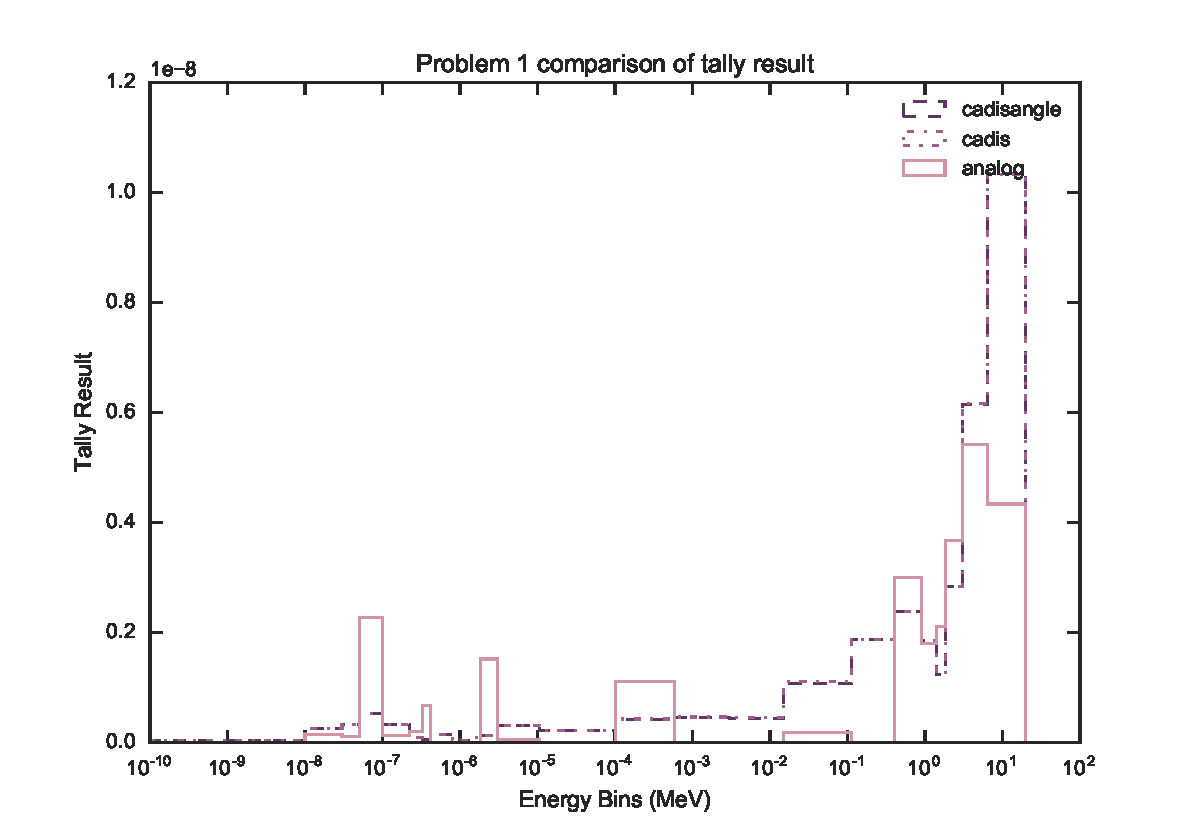
\includegraphics[height=10cm]{./chapters/characterization_probs/figures/char/prob_1/problem_1_tally_result_compare.pdf}
  \caption[Tally results comparison between methods for steel bar embedded in
  concrete.]
  {Tally results comparison between methods for steel bar embedded in concrete.}
  \label{fig:steelbeamresult}
\end{figure}

\begin{figure}[h!]
  \centering
  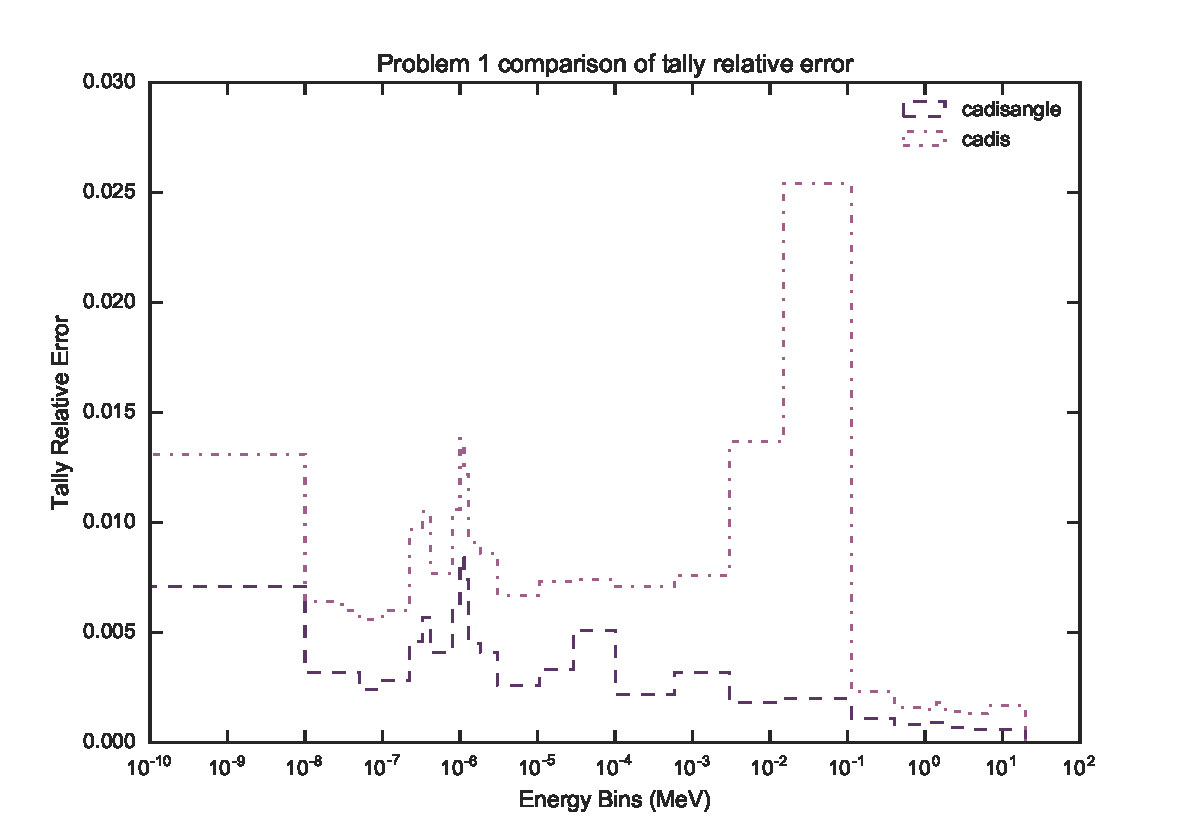
\includegraphics[height=10cm]{./chapters/characterization_probs/figures/char/prob_1/problem_1_tally_error_compare.pdf}
  \caption[Tally relative error comparison between methods for steel bar
  embedded in concrete.]
  {Tally relative error comparison between methods for steel bar embedded in
  concrete.}
  \label{fig:steelbeamerror}
\end{figure}

Figure \ref{fig:steelbeamresult} shows that CADIS and CADIS-$\Omega$ are in
agreement for the tally results in all energy bins. The nonbiased Monte Carlo
calculation differs from both of the hybrid methods. This supports what was
observed in the nonbiased analog FOM values of Table \ref{tab:steelbeamfoms}.
Figure
\ref{fig:steelbeamerror} shows that CADIS-$\Omega$ achieves a
consistently lower relative error than CADIS for all energy bins. For most
energy bins, CADIS-$\Omega$'s relative errors are shifted a consistent fraction
below CADIS'. In the energy regions between $10^{-4}$ and $10^{-1}$ MeV, this is
not the case. For these energy regions CADIS' relative errors spike while
CADIS-$\Omega$'s do not.

% [add anisotropy plots here]
%
% [describe why anisotropy might have happened in this region]
%
% [make visit plot of problematic energy group in adjoint flux and omega flux.
% compare and discuss differences.]

From the FOM results presented in Table \ref{tab:steelbeamfoms} and the tally
results and error in Figures \ref{fig:steelbeamresult} and
\ref{fig:steelbeamerror}, we can conclude that
CADIS-$\Omega$'s source biasing parameters consistently move more particles in
all tally energy bins more effectively than CADIS.
The importance map generated by CADIS-$\Omega$
better reflects the problem physics and more efficiently transports particles to
the desired tally location.

\subsubsection{Air Channel Variant}
\label{subsubsec:airbeam}

The characterization problems have been designed to induce anisotropy in
the flux. Most of these problems do so, in some part, by using air to induce
particle streaming. The steel beam in concrete problem requires that particles
interact with a high density material (either steel or concrete) before reaching
the detector to induce a response. These next two variant problems explore
whether the material choice of steel strongly affects the $\Omega$-method's
ability to generate variance reduction parameters. This first variant keeps the
geometric configuration of the steel beam problem the same, but the steel is
replaced with air. If the $\Omega$-methods are more sensitive to air, then this
change in the materials composition should affect the results.

\begin{table}[h!]
  \centering
  \begin{tabular}{lrrrrr}
\toprule
{} & cadis &             & cadisangle &             & analog \\
{} &    MC & MC\_adjusted &         MC & MC\_adjusted &     MC \\
\midrule
tally avg   &   432 &         390 &        396 &         364 &   5.63 \\
max RE      &  1.17 &        1.05 &      0.247 &       0.227 & 0.0467 \\
min RE      &   273 &         247 &        296 &         272 &    -- \\
time (mins) &  47.3 &        52.3 &        247 &         268 &   21.4 \\
\bottomrule
\end{tabular}

  \caption[Figure of Merit comparison for the air variant of the steel beam
  problem geometry.]
  {Figure of Merit comparison for air variant of the steel beam problem geometry. In this
  variant problem, the steel bar volume region is replaced with air to
exacerbate the suggested splitting issues encountered in other hybrid problems. }
  \label{tab:airbeamfoms}
\end{table}

\begin{table}[h!]
  \centering
  \begin{tabular}{llrrr}
\toprule
          &              &          cadis &     cadisangle &         analog \\
          &              & time (minutes) & time (minutes) & time (minutes) \\
\midrule
MCNP time & total &          47.29 &         246.83 &          21.42 \\
deterministic time & advantg\_time &           0.16 &           0.15 &            -- \\
          & denovo\_time &           4.90 &          20.50 &            -- \\
          & dispose\_time &           0.00 &           0.15 &            -- \\
          & omega\_time &           0.00 &           0.65 &            -- \\
          & total &           5.05 &          21.30 &            -- \\
wall time &              &          52.34 &         268.13 &          21.42 \\
\bottomrule
\end{tabular}

  \caption[Detailed timing results for steel beam geometry air variant.]
  {Detailed timing results for steel beam geometry air variant.}
  \label{tab:airbeamtimes}
\end{table}

Tables \ref{tab:airbeamfoms} and \ref{tab:airbeamtimes} summarize the FOM and timing
results for the air variant of the steel beam problem. Comparing the FOMs for
this variant and for the steel variant (Table \ref{tab:steelbeamfoms}), it is
clear that CADIS-$\Omega$ performs more poorly than CADIS with air.
Interestingly, CADIS-$\Omega$'s minimum relative error FOM is better than
CADIS', which is opposite to the results for the standard steel problem. For the
maximum relative error, CADIS-$\Omega$'s FOM is 1/5th that of CADIS'. However,
for this problem CADIS-$\Omega$'s runtime is almost five times that of CADIS.
Considering this time difference, it appears that CADIS-$\Omega$ requires far
more sampling with its importance map than CADIS. These sampling requirements
also exist with the original steel problem, but the importance map reduces the
tally variance enough to offset the time addition. This is not the case for the
air variant. From this, we can conclude that the addition of air into this
problem geometry reduces the sampling interaction points enough to negatively
affect the $\Omega$-method. Further, it lowers the FOMs achieved by both CADIS
and CADIS-$\Omega$ substantially that their improvement over the nonbiased
analog reduces almost an order of magnitude.

The runtimes in Table \ref{tab:airbeamtimes} are also worth comparing with the
original steel variant. In particular, the deterministic runtime in both of the
promblems is on the same order of magnitude. However, the Monte Carlo runtime is
far longer in the original steel version. The runtimes in the air variant are
generally much shorter for CADIS and CADIS-$\Omega$, but comparable for the
nonbiased analog. In this problem, the fraction of time spent in the
deterministic solve is much higher than in the steel version.

\subsubsection{Concrete Channel Variant}
\label{subsubsec:concretebeam}

In addition to the air variant of the steel beam geometry, we can see if having
non-preferential flowpaths might affect the $\Omega$-method's performance.
Recall that the $\Omega$-methods have been designed to incorporate angular
information into the importance map. If no preferential flowpaths exist through
the problem geometry, then the $\Omega$-importance map may have less of an
impact on improving the tally convergence. However, because the entire shield is
composed of concrete, then the distance to smapling location should still be
quite small as with the original steel version of the problem. As a result, there
should be some positive effects on the $\Omega$-methods due to sampling
interaction frequency. Tables \ref{tab:concretebeamfoms} and
\ref{tab:concretebeamtimes} show the FOM and timing results for this material
variant of the steel beam geometry.

\begin{table}[h!]
  \centering
  \begin{tabular}{lrrrrr}
\toprule
{} &    cadis &             & cadisangle &             & analog \\
{} &       MC & MC\_adjusted &         MC & MC\_adjusted &     MC \\
\midrule
tally avg   &  2.6e+03 &    2.55e+03 &   3.16e+03 &    3.13e+03 &   1.54 \\
max RE      &     14.5 &        14.2 &       9.48 &        9.39 & 0.0457 \\
min RE      & 1.54e+03 &    1.51e+03 &    1.4e+03 &    1.39e+03 &    -- \\
time (mins) &      385 &         393 &   1.98e+03 &       2e+03 &   21.9 \\
\bottomrule
\end{tabular}

  \caption[Figure of Merit comparison for concrete variant of steel bar geometry.]
  {Figure of Merit comparison for concrete variant of steel bar geometry. In this
  variant problem, the steel bar volume region is replaced with concrete to
  eliminate the preferential particle travel through the beam region.}
  \label{tab:concretebeamfoms}
\end{table}

\begin{table}[h!]
  \centering
  \begin{tabular}{llrrr}
\toprule
          &              &          cadis &     cadisangle &         analog \\
          &              & time (minutes) & time (minutes) & time (minutes) \\
\midrule
MCNP time & total &         385.11 &        1978.46 &          21.88 \\
deterministic time & advantg\_time &           0.23 &           0.15 &            -- \\
          & denovo\_time &           7.42 &          19.58 &            -- \\
          & dispose\_time &           0.00 &           0.09 &            -- \\
          & omega\_time &           0.00 &           0.56 &            -- \\
          & total &           7.65 &          20.29 &            -- \\
wall time &              &         392.76 &        1998.75 &          21.88 \\
\bottomrule
\end{tabular}

  \caption[Detailed timing results for concrete variant of steel bar.]
  {Detailed timing results for concrete variant of steel bar.}
  \label{tab:concretebeamtimes}
\end{table}

Tables \ref{tab:concretebeamfoms} and \ref{tab:concretebeamtimes} show the
results of the concrete variant of the steel beam problem. As with the original
steel and air versions described previously, the runtimes for CADIS-$\Omega$ are quite
long when compared to CADIS. In each variant, the runtimes are about five times
longer than those observed for CADIS. Similarly to the steel variant, in this
version CADIS-$\Omega$ achieves a superior FOM for the tally average FOM.
However, CADIS-$\Omega$'s FOMS for the maximum and minimum relative error FOMs
are both lower than CADIS'. Both CADIS and CADIS-$\Omega$ far outperform the
nonbiased analog Monte Carlo.

\subsection{U-Shaped Corridor}
\label{subsec:resultsucorridor}

The U-shaped air corridor embedded in concrete
FOM and timing
results are summarized in Tables
\ref{tab:ucorridorfoms} and \ref{tab:ucorridortimes}. Figures
\ref{fig:ucorridorresult} and \ref{fig:ucorridorerror} show the results obtained
by the track length tally in CADIS, CADIS-$\Omega$ and the nonbiased analog
Monte Carlo.

\begin{table}[h!]
  \centering
  \begin{tabular}{lrrrrr}
\toprule
{} &  cadis &             & cadisangle &             & analog \\
{} &     MC & MC\_adjusted &         MC & MC\_adjusted &     MC \\
\midrule
tally avg   &   64.1 &        51.9 &       60.2 &        38.3 &  0.378 \\
max RE      & 0.0183 &      0.0148 &     0.0144 &     0.00913 & 0.0644 \\
min RE      &   14.9 &          12 &       13.4 &        8.54 &    -- \\
time (mins) &   54.6 &        67.5 &        188 &         296 &   15.5 \\
\bottomrule
\end{tabular}

  \caption[Figure of Merit comparison between methods for U-shaped air corridor in concrete.]
  {Figure of Merit comparison between methods for U-shaped air corridor in
  concrete.}
  \label{tab:ucorridorfoms}
\end{table}

\begin{table}[h!]
  \centering
  \begin{tabular}{llrrr}
\toprule
          &             &          CADIS & CADIS-$\Omega$ &         analog \\
        &              & \multicolumn{3}{c}{time (minutes)} \\
\midrule
MCNP time & total &          54.61 &         187.92 &          15.54 \\
deterministic time & advantg\_time &           0.19 &           0.21 &            -- \\
          & denovo\_time &          12.68 &         105.90 &            -- \\
          & dispose\_time &           0.01 &           0.35 &            -- \\
          & omega\_time &           0.00 &           1.49 &            -- \\
          & total &          12.87 &         107.60 &            -- \\
wall time &              &          67.48 &         295.52 &          15.54 \\
\bottomrule
\end{tabular}

  \caption[Detailed timing results for U-shaped air corridor in concrete.]
  {Detailed timing results for U-shaped air corridor in concrete.}
  \label{tab:ucorridortimes}
\end{table}

Much like the single- and multiple-turn labyrinths, the U-shaped air corridor
has a pathway of preferential movement for particles in a concrete shield. In
this problem, the particles travel down the legs of the u-bend to a detector on
the other side of the corridor. The particles should have preferential flowpaths
through the air ducts, but it is possible for low energy particles to traverse
the concrete barrier between the source and detector. The high energy particles
tallied in the detector are more likely to have traveled through the air ducts
and the low energy particles may be supplied from the shield or from scattering
down the air duct.

The FOM table for the u-shaped corridor shows that this is a fairly difficult
problem for CADIS, CADIS-$\Omega$, and the analog. For the tally average FOM,
CADIS and CADIS-$\Omega$ achieve a FOM two orders of magnitude higher than the
nonbiased analog. Both methods have comparable FOMs. In fact, CADIS and
CADIS-$\Omega$ are in relative agreement for all FOMs calculated with the Monte
Carlo runtime. Interestingly, the nonbiased analog Monte Carlo has a higher
maximum relative error FOM than either method. However, this analog tally for
this problem has many
nontallied bins (as can be gathered from the major discrepancy in results in
Figures \ref{fig:ucorridorresult} and \ref{fig:ucorridorerror}). For the
few bins that were tallied, the analog has a high FOM.

\begin{figure}[h!]
  \centering
  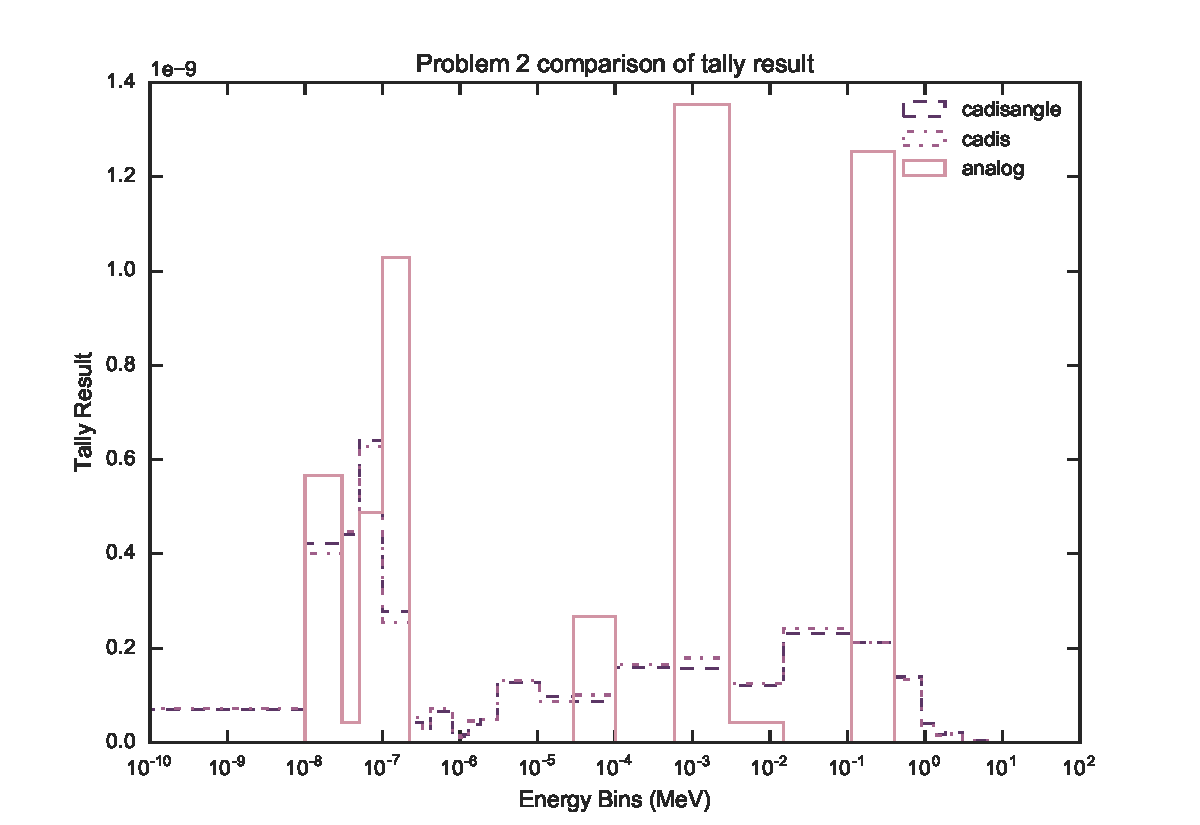
\includegraphics[height=10cm]{./chapters/characterization_probs/figures/char/prob_2/problem_2_tally_result_compare.pdf}
  \caption[Tally results comparison between methods for U-shaped air corridor in
  concrete.]
  {Tally results comparison between methods for U-shaped air corridor in
  concrete.}
  \label{fig:ucorridorresult}
\end{figure}

\begin{figure}[h!]
  \centering
  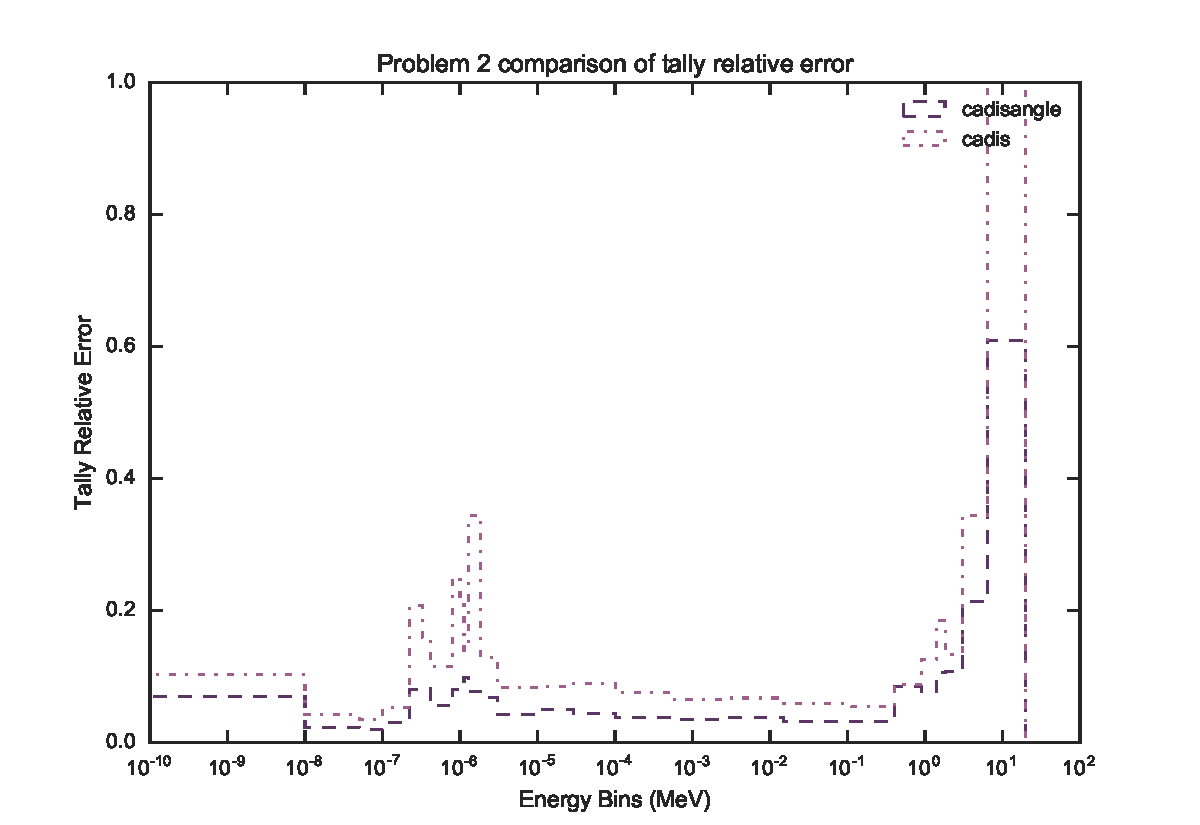
\includegraphics[height=10cm]{./chapters/characterization_probs/figures/char/prob_2/problem_2_tally_error_compare.pdf}
  \caption[Tally relative error comparison between methods for U-shaped air
  corridor in concrete.]
  {Tally relative error comparison between methods for U-shaped air corridor in
  concrete.}
  \label{fig:ucorridorerror}
\end{figure}

The tally results for the u-shaped corridor in Figure \ref{fig:ucorridorresult}
show general agreement between CADIS and CADIS-$\Omega$. The nonbiased analog
has no agreement with either method. Comparing their relative errors in Figure
\ref{fig:ucorridorerror}, we can gather that this is a difficult problem for
both methods. At high energies both CADIS and CADIS-$\Omega$ have very high
relative errors, indicating untrustworthy results. To get the relative error in
these regions for CADIS-$\Omega$ to below 0.10--a fairly standard threshold for
Monte Carlo--it would have to run nearly 40x longer, or ~900 hours. However,
CADIS-$\Omega$ achieves a uniformly lower relative error than CADIS for all
energy bins. Because the time to run CADIS-$\Omega$ is so much longer, the FOM
is impacted and appears worse than CADIS. Therefore, should CADIS-$\Omega$ use
the same runtime as CADIS, CADIS will achieve superior relative errors.
Conversely, if CADIS-$\Omega$ uses the same particle count as CADIS,
CADIS-$\Omega$ will achieve superior relative errors.

\subsection{Shielding with Rebar}
\label{subsec:resultrebar}

The problem with rebar embedded both in the x- and y- directions
in concrete has
results summarized in Tables
\ref{tab:rebarfoms} and \ref{tab:rebartimes}. Figures
\ref{fig:rebarresult} and \ref{fig:rebarerror} show the results obtained
by the track length tally in CADIS, CADIS-$\Omega$ and the nonbiased analog
Monte Carlo.

\begin{table}[h!]
  \centering
  \begin{tabular}{lrrrrr}
\toprule
{} & \multicolumn{2}{c}{CADIS}   & \multicolumn{2}{c}{CADIS-$\Omega$}  & analog \\
{} &    MC & MC$_{hybrid}$ &         MC & MC$_{hybrid}$ &     MC \\
\midrule
tally avg   &   1.15 &        1.09 &     0.0136 &      0.0127 &  0.948 \\
max RE      & 0.0345 &      0.0327 &    0.00117 &     0.00109 & 0.0186 \\
min RE      &    235 &         223 &        199 &         186 &    -- \\
time (mins) &    328 &         346 &   1.55e+03 &    1.66e+03 &   53.8 \\
\bottomrule
\end{tabular}

  \caption[Figure of Merit comparison between methods for rebar-embedded
  concrete.]{Figure of Merit comparison between methods for rebar-embedded
  concrete.}
  \label{tab:rebarfoms}
\end{table}

\begin{table}[h!]
  \centering
  \begin{tabular}{llrrr}
\toprule
          &              &          cadis &     cadisangle &         analog \\
          &              & time (minutes) & time (minutes) & time (minutes) \\
\midrule
MCNP time & total &         327.81 &        1550.54 &          53.82 \\
deterministic time & advantg\_time &           0.28 &           0.29 &            -- \\
          & denovo\_time &          17.70 &         105.09 &            -- \\
          & dispose\_time &           0.03 &           0.41 &            -- \\
          & omega\_time &           0.00 &           2.05 &            -- \\
          & total &          17.98 &         107.43 &            -- \\
wall time &              &         345.79 &        1657.97 &          53.82 \\
\bottomrule
\end{tabular}

  \caption[Detailed timing results for rebar-embedded concrete]
  {Detailed timing results for rebar-embedded concrete.}
  \label{tab:rebartimes}
\end{table}

The FOM results for the rebar-embedded concrete show that this is a very poor
problem for CADIS-$\Omega$, in general. CADIS-$\Omega$ has lower FOMs than CADIS
in all measures. CADIS-$\Omega$ spends fractionally over five--both
deterministically and in Monte Carlo--the
transport time that CADIS does. Further, CADIS-$\Omega$ has poorer FOMs in both
the tally average and maximum relative error than the nonbiased analog. This is
due to CADIS-$\Omega$ requiring nearly 30x longer to run Monte Carlo than the
nonbiased analog.

\begin{figure}[h!]
  \centering
  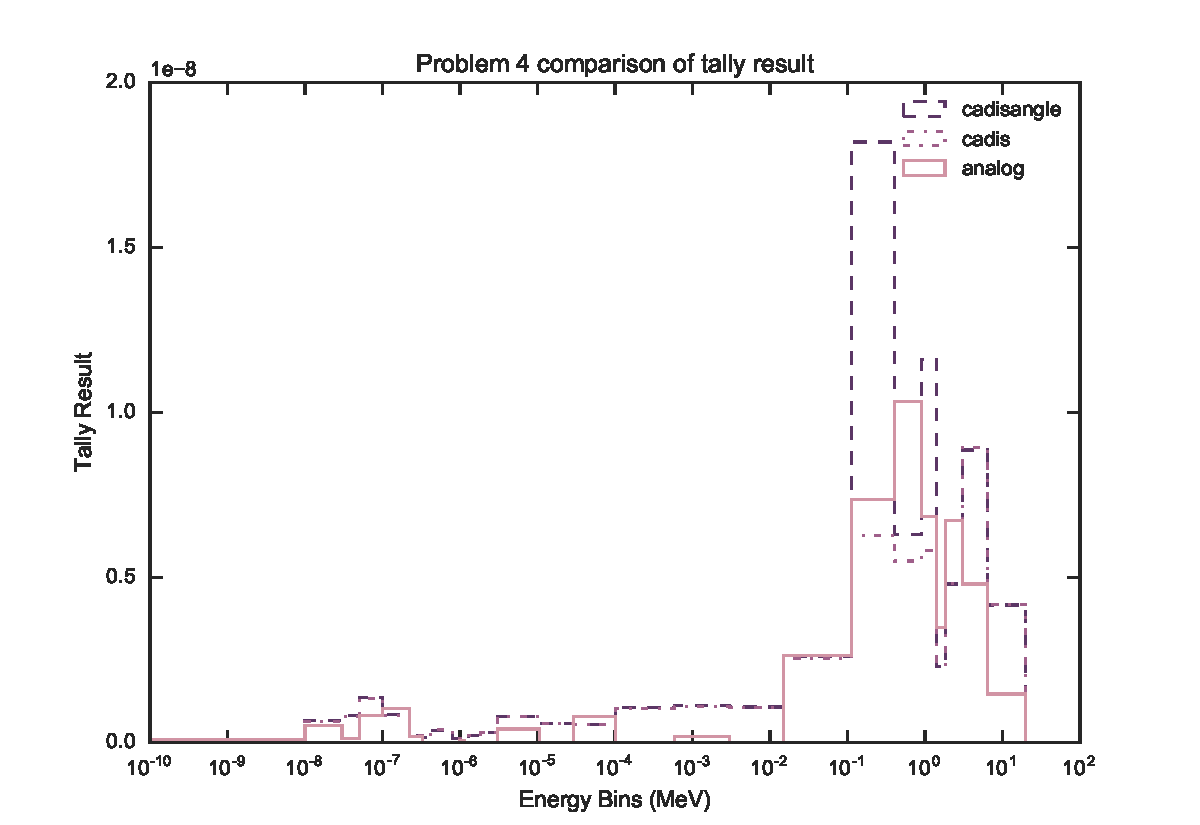
\includegraphics[height=10cm]{./chapters/characterization_probs/figures/char/prob_4/problem_4_tally_result_compare.pdf}
  \caption[Tally results comparison between methods for rebar-embedded concrete.]
  {Tally results comparison between methods for rebar-embedded concrete.}
  \label{fig:rebarresult}
\end{figure}

\begin{figure}[h!]
  \centering
  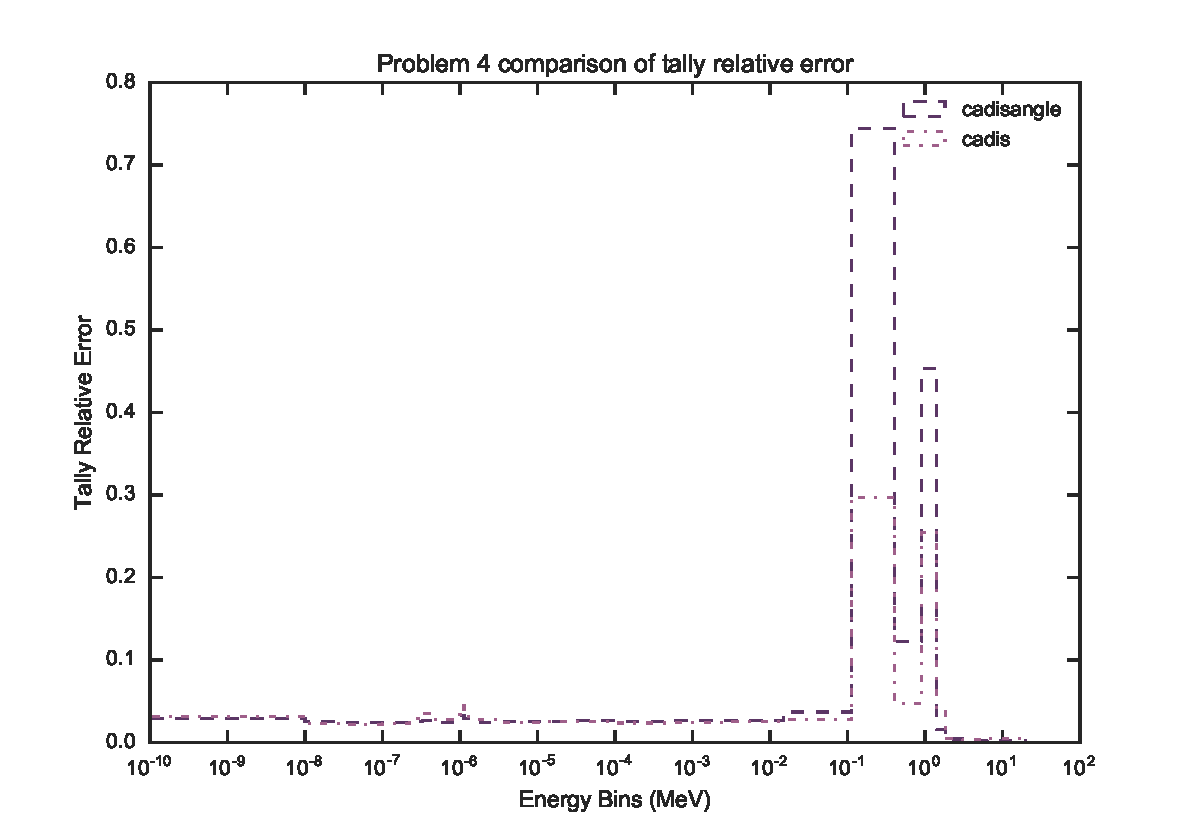
\includegraphics[height=10cm]{./chapters/characterization_probs/figures/char/prob_4/problem_4_tally_error_compare.pdf}
  \caption[Tally relative error comparison between methods for rebar-embedded concrete.]
  {Tally relative error comparison between methods for rebar-embedded concrete.}
  \label{fig:rebarerror}
\end{figure}

Figure \ref{fig:rebarresult} shows that the tally results for the rebar-embedded
concrete do not generally agree between any method. CADIS and CADIS-$\Omega$
have better agreement with each other than with the nonbiased analog, but at
high energies their results differ significantly. However, in comparing their
relative errors in Figure \ref{fig:rebarerror}, the large discrepancy in their
results is explained by the very high relative errors in this region. As with
the u-shaped air corridor, neither method achieves satisfactory relative errors
below 0.10 in high energy bins. However, both methods achieve comparitavely good
relative error results in energy bins below $10^{-1}$ MeV.

Unlike previous problems that had
significant problem volumes filled with air, this particular problem has a thick
shield with which incident particles must interact. While this problem may
appear similar geometrically to the beam embedded in
concrete, this problem has far more preferential flowpaths by which particles
might flow. Some of these flowpaths are directed perpindicularly to a path
towards the detector. It is possible that CADIS-$\Omega$ is capturing these
flowpaths, but because they are not towards the detector CADIS-$\Omega$ spends a
significant portion of its time sampling less useful regions.

\subsection{Beam Problem}
\label{subsec:resultsbeam}

The nuclear physics beamline toy problem has FOM and timing
results summarized in Tables
\ref{tab:beamfoms} and \ref{tab:beamtimes}. Figures
\ref{fig:beamresult} and \ref{fig:beamerror} show the results obtained
by the track length tally in CADIS, CADIS-$\Omega$ and the nonbiased analog
Monte Carlo.

\begin{table}[h!]
  \centering
  \begin{tabular}{lrrrrr}
\toprule
{} & cadis &             & cadisangle &             & analog \\
{} &    MC & MC\_adjusted &         MC & MC\_adjusted &     MC \\
\midrule
tally avg   &   368 &         138 &       94.8 &        7.91 &    317 \\
max RE      & 0.542 &       0.202 &       1.18 &      0.0984 &    1.6 \\
min RE      &   -- &         -- &        -- &         -- &    -- \\
time (mins) &  2.23 &        5.97 &       1.69 &        20.3 &   1.69 \\
\bottomrule
\end{tabular}

  \caption[Figure of Merit comparison between methods for simplified
    experimental nuclear physics beamline.]
    {Figure of Merit comparison between methods for simplified experimental
    nuclear physics beamline.}
  \label{tab:beamfoms}
\end{table}

\begin{table}[h!]
  \centering
  \begin{tabular}{llrrr}
\toprule
          &             &          CADIS & CADIS-$\Omega$ &         analog \\
        &              & \multicolumn{3}{c}{time (minutes)} \\
\midrule
MCNP time & total &           2.23 &           1.69 &           1.69 \\
deterministic time & advantg\_time &           0.17 &           0.15 &            -- \\
          & denovo\_time &           3.57 &          17.88 &            -- \\
          & dispose\_time &           0.00 &           0.12 &            -- \\
          & omega\_time &           0.00 &           0.53 &            -- \\
          & total &           3.74 &          18.56 &            -- \\
wall time &              &           5.97 &          20.25 &           1.69 \\
\bottomrule
\end{tabular}

  \caption[Detailed timing results for simplified experimental nuclear physics
  beamline.]
  {Detailed timing results for simplified experimental nuclear physics beamline.}
  \label{tab:beamtimes}
\end{table}

The experimental nuclear physics beamline problem is the most
difficult of the characterization problems for both CADIS and CADIS-$\Omega$.
There are no walls off which
particles may scatter; the only places most particles will scatter is in the
detector regions and potentially off of air. These particular problems were run
with $1e9$ particles rather than $1e7$. Because there are so few interaction
points, the majority of particles leak out of the problem boundary so
more source particles are required to obtain results.

Table \ref{tab:beamfoms} shows that nuclear physics experimental beamline
problem has very slow convergence for
CADIS and CADIS-$\Omega$. CADIS, CADIS-$\Omega$ and the nonbiased analog all have
zero-scoring tally bins. These are in low energy regions, energy regions in
which particles in the problem never reach.
The maximum relative error FOM for CADIS, CADIS-$\Omega$,
and the nonbiased analog are all very low, indicating that the threshold for
convergence of the highest energy bin will take a long time for all three
methods. Interestingly, CADIS performs worse than CADIS-$\Omega$ and the
nonbiased analog with this metric. The nonbiased analog achieves the highest
maximum relative error FOM and the highest tally average relative error FOM for all
three methods.

A notable feature of Table \ref{tab:beamtimes} is the Monte Carlo runtime of
CADIS, CADIS-$\Omega$, and the nobiased analog. In previous characterization
problems, CADIS-$\Omega$ and CADIS had much longer runtimes than the nonbiased
analog. In all of the previous characterization problems, CADIS-$\Omega$ had a
longer runtime than CADIS. In this problem, CADIS-$\Omega$ has a shorter runtime
than CADIS. The deterministic runtime of CADIS-$\Omega$ relative to CADIS
is comparable to previous problems. A potential reason that the runtimes of
CADIS and CADIS-$\Omega$ is so close to the nonbiased analog is because so many
particles leak out of the problem space.
% Further, the reason that CADIS-$\Omega$
% may have a shorter runtime than CADIS is because ray effects are dampened in the
% problem. As a result, unphysical fluctuations in the flux that may generate
% additional sampling issues are eliminated with CADIS-$\Omega$.

\begin{figure}[h!]
  \centering
  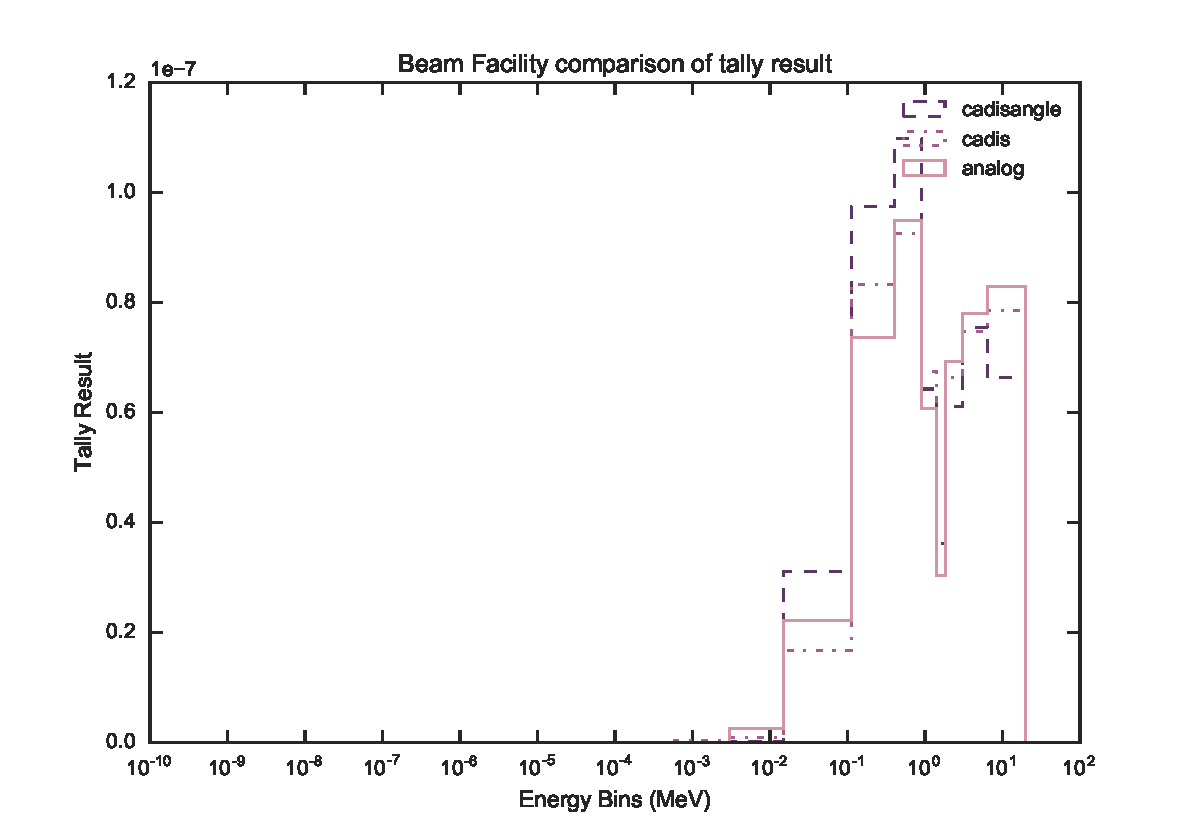
\includegraphics[height=10cm]{./chapters/characterization_probs/figures/char/beam/beam_facility_tally_result_compare.pdf}
  \caption[Tally results comparison between methods for simplified experimental
    nuclear physics beamline.]
  {Tally results comparison between methods for simplified experimental
    nuclear physics beamline.}
  \label{fig:beamresult}
\end{figure}

\begin{figure}[h!]
  \centering
  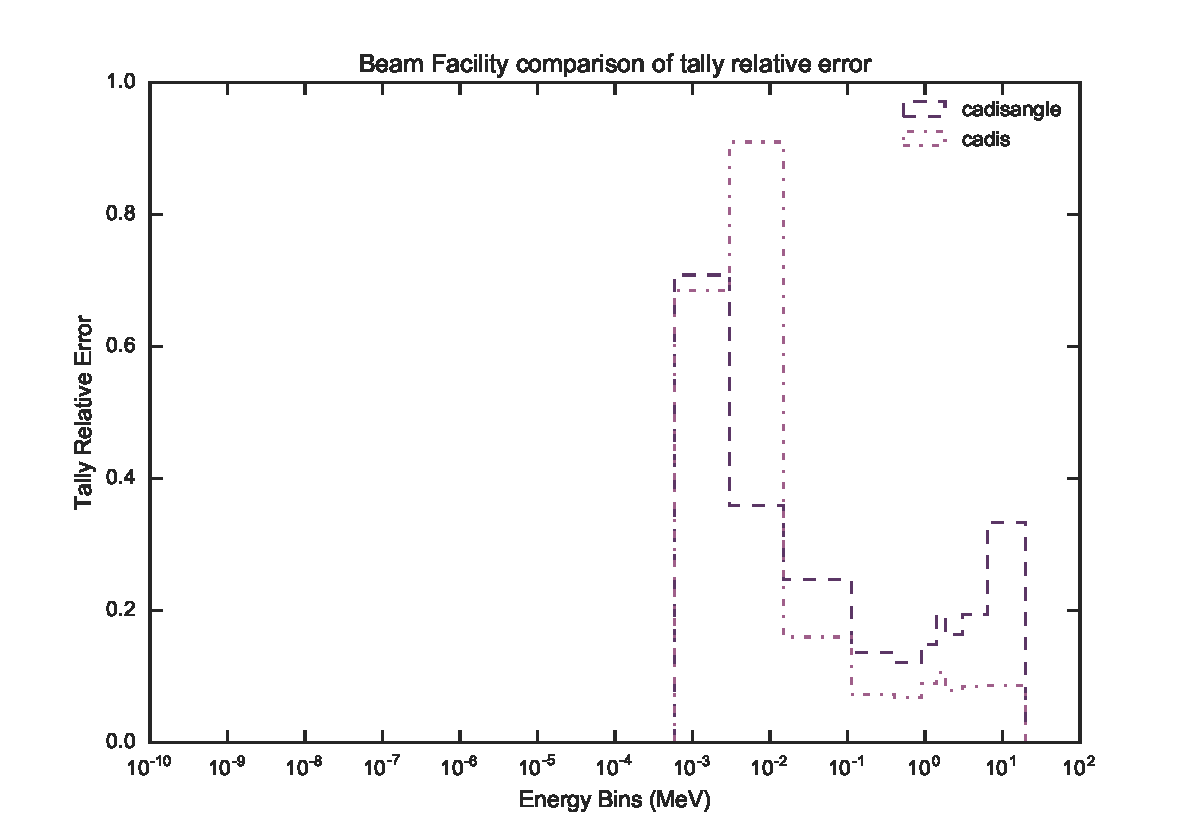
\includegraphics[height=10cm]{./chapters/characterization_probs/figures/char/beam/beam_facility_tally_error_compare.pdf}
  \caption[Tally relative error comparison between methods
    for simplified experimental nuclear physics beamline.]
  {Tally relative error comparison between methods for simplified experimental
    nuclear physics beamline.}
  \label{fig:beamerror}
\end{figure}

Comparing the full tally results presented in Figures \ref{fig:beamresult} and
\ref{fig:beamerror}, the FOM results from Table \ref{tab:beamfoms} have more
context. Figure \ref{fig:beamresult} shows that all three methods have similar
results in the track length tally. In a few of the bins CADIS and the nonbiased
analog appear to have closer results than CADIS and CADIS-$\Omega$.

\subsection{Therapy Room}
\label{subsec:resultstherapy}

The problem with a simplified representation of a nuclear medicine therapy room
has FOM and timing
results summarized in Tables
\ref{tab:therapyfoms} and \ref{tab:therapytimes}. Figures
\ref{fig:therapyresult} and \ref{fig:therapyerror} show the results obtained
by the track length tally in CADIS, CADIS-$\Omega$ and the nonbiased analog
Monte Carlo. Note that the results for this problem had issues with reported
times for the deterministic run, so the adjusted Monte Carlo
(FOM$_{hybrid}$) is not reported and the timing table is not reported.

\begin{table}[h!]
  \centering
  \begin{tabular}{lrrrrr}
\toprule
{} & cadis &             & cadisangle &             & analog \\
{} &    MC & MC\_adjusted &         MC & MC\_adjusted &     MC \\
\midrule
tally avg   &  5.81 &        5.71 &        106 &        8.34 &   2.81 \\
max RE      & 0.463 &       0.455 &      0.822 &      0.0649 & 0.0136 \\
min RE      &  37.6 &          37 &       32.9 &         2.6 &  0.793 \\
time (mins) &  44.7 &        45.4 &       39.9 &         506 &    248 \\
\bottomrule
\end{tabular}

  \caption[Tally results comparison between methods for simplified medical
  therapy room.]{Tally relative error comparison between methods for simplified
  medical therapy room.}
  \label{tab:therapyfoms}
\end{table}

% \begin{table}[h!]
%   \centering
%   \begin{tabular}{llrrr}
\toprule
          &              &          cadis &     cadisangle &         analog \\
          &              & time (minutes) & time (minutes) & time (minutes) \\
\midrule
MCNP time & total &          44.66 &          39.92 &          248.0 \\
deterministic time & advantg\_time &           0.62 &           0.91 &            -- \\
          & denovo\_time &           0.17 &         438.05 &            -- \\
          & dispose\_time &           0.00 &          24.76 &            -- \\
          & omega\_time &           0.00 &          26.63 &            -- \\
          & total &           0.79 &         465.58 &            -- \\
wall time &              &          45.45 &         505.50 &          248.0 \\
\bottomrule
\end{tabular}

%   \caption[Tally relative error comparison between methods for simplified
%   medical therapy room.]{Tally relative error comparison between methods for
%   simplified medical therapy room.}
%   \label{tab:therapytimess}
% \end{table}




\begin{figure}[h!]
  \centering
  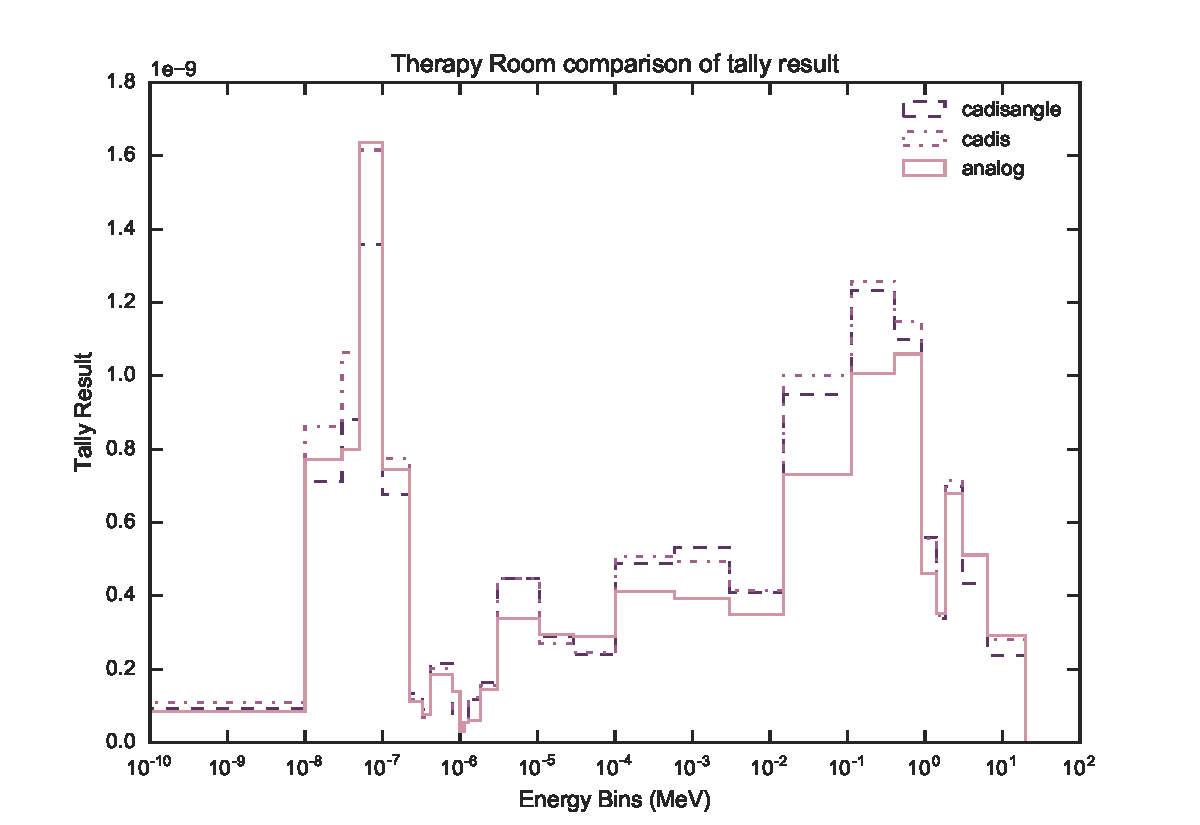
\includegraphics[height=10cm]{./chapters/characterization_probs/figures/char/therapy/therapy_room_tally_result_compare.pdf}
  \caption[Tally results comparison between methods for simplified medical
  therapy room.]
  {Tally results comparison between methods for simplified medical therapy room.}
  \label{fig:therapyresult}
\end{figure}

\begin{figure}[h!]
  \centering
  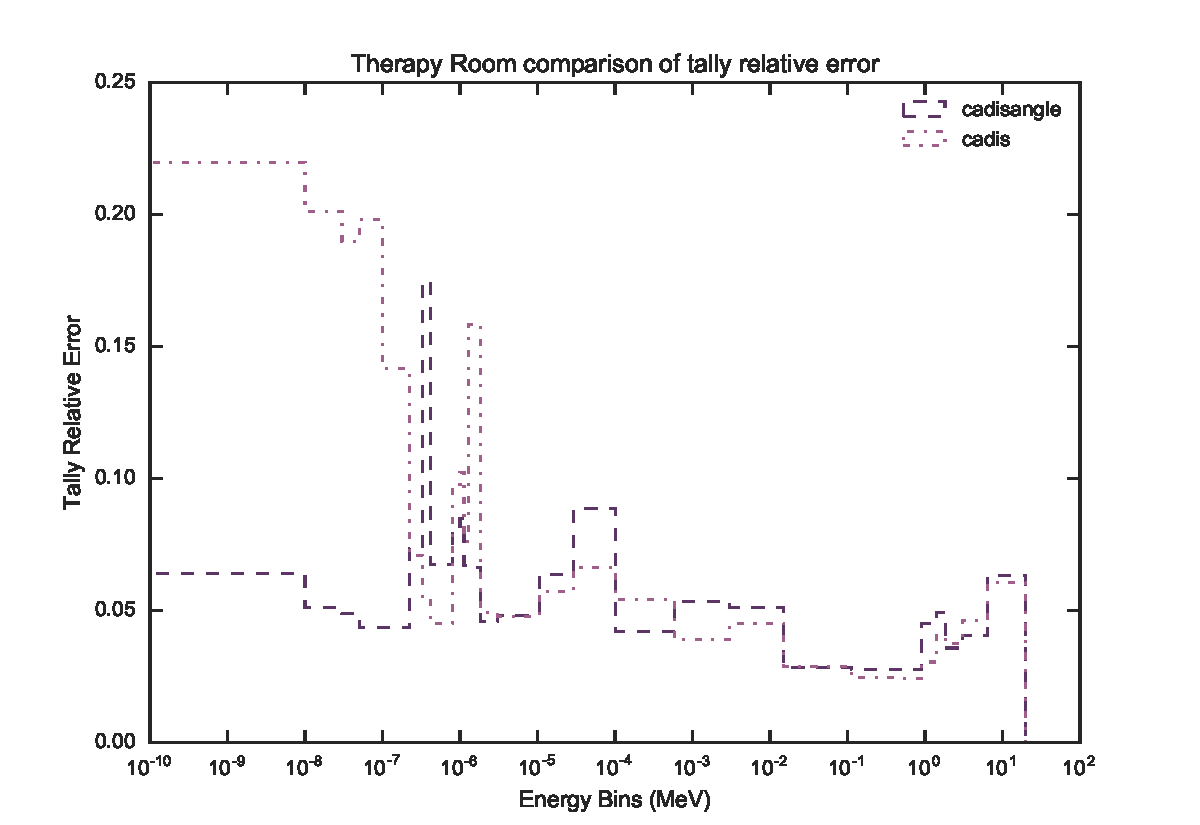
\includegraphics[height=10cm]{./chapters/characterization_probs/figures/char/therapy/therapy_room_tally_error_compare.pdf}
  \caption[Tally relative error comparison between methods for simplified
  medical therapy room.]
  {Tally relative error comparison between methods for simplified medical
  therapy room.}
  \label{fig:therapyerror}
\end{figure}

